% This file should be replaced with your file with an thesis content.
%=========================================================================
% Authors: Michal Bidlo, Bohuslav Křena, Jaroslav Dytrych, Petr Veigend and Adam Herout 2019

\definecolor{darkpastelred}{rgb}{0.76, 0.23, 0.13}
\definecolor{codegreen}{rgb}{0,0.6,0}
\definecolor{codegray}{rgb}{0.5,0.5,0.5}
\definecolor{codepurple}{rgb}{0.58,0,0.82}
\definecolor{backcolour}{rgb}{0.95,0.95,0.92}
\lstset{
    string=[s]{"}{"},
    stringstyle=\color{darkpastelred},
    comment=[l]{:},
    commentstyle=\color{black},
    caption=Example of event described using CloudEvents specification and JSON
}


\lstdefinestyle{jsonStyle}{
    string=[s]{"}{"},
    stringstyle=\color{darkpastelred},
    comment=[l]{:},
    breaklines=true,
    commentstyle=\color{black}
}

\lstdefinestyle{pythonStyle}{
    backgroundcolor=\color{backcolour},
    commentstyle=\color{codegreen},
    keywordstyle=\color{blue},
    numberstyle=\tiny\color{codegray},
    stringstyle=\color{codepurple},
    basicstyle=\ttfamily\footnotesize,
    breakatwhitespace=false,
    breaklines=true,
    captionpos=b,
    keepspaces=true,
    numbers=left,
    showspaces=false,
    showstringspaces=false,
    showtabs=false,
    tabsize=2
}

\newenvironment{customlegend}[1][]{%
    \begingroup
    \csname pgfplots@init@cleared@structures\endcsname
    \pgfplotsset{#1}%
}{%
    \csname pgfplots@createlegend\endcsname
    \endgroup
}%
\def\addlegendimage{\csname pgfplots@addlegendimage\endcsname}

\hyphenation{OpenStack Swift OpenIO SDS}

\chapter{Introduction}\label{chap:introduction}

% general introduction for a topic:
%- cloud computing popularity
%- most popular service: cloud storage and its types
%- about object storage
%- users interest of what's going in theirs storage / event activities
%- TODO: maybe remove talk about types of cloud storages? solution: talk about need for monitoring and users need to monitor/receive information regarding their storage
In the current world, cloud computing has become the most popular way of delivering different services on the Internet. One of the most popular cloud services is cloud storage, allowing users to store data in remote locations maintained by a third party. Based on how cloud storage manages data, cloud storage can be divided into three types: Block storage, File storage, and Object storage. Object storage manages data as objects, and each object typically includes data itself and some additional information stored in object metadata. Since data are stored in remote locations, to which users do not have direct and complete access, some users or external services might want to receive information about specific events (for example, change of content) in storages where their data are located.

% importance of thesis in this field
%- react to events - possibly react to 'bad' events
%- allows users to have a better picture of what is going on in their storage
The importance of this thesis is to provide event information to users in OpenIO SDS and OpenStack Swift, which will allow users to react to those events, create more sophisticated backend operations and postprocessing, or possibly prevent/detect unwanted actions. In addition, providing event notifications will allow users to have a better picture of what is going on in their storage and improve monitoring in these object storages.

%past advances in this field
There were two attempts\cite{swiftPatch1}\cite{swiftPatch2} to solve this issue within OpenStack Swift which were not officially accepted, and their solution is outdated. So currently, there is no official solution for publishing event notifications in OpenStack Swift nor OpenIO Software-Defined Storage (from now on SDS).

%why am I interested in this, why I choose this topic
%- perosnally i used object storage
%- can se myself using this solution in future as well as millions of other users
%- impact on big amount of users
%- contibuting to open source projects
My interest in this topic stems from its possible impact on the extensive amount of users that OpenStack Swift and OpenIO have. Furthermore, I have always wanted to contribute to open-source projects. The possibility to improve user experience in OpenStack Swift and OpenIO SDS and allow these storags to be even more competitive against commercial storage (Amazon, Google, ...) is another reason why I choose this topic.

%goals of thesis
This thesis aims to create a program/middleware which will publish event notifications to user-specified destinations. One of the supported destinations will be the Beanstalk queue, but the program can be easily configured to support other destinations (for example, Kafka) using a predefined interface. The proposed program will allow users to specify, using object metadata (such as name prefix/suffix and object size) and type of event, which event notification should be published. The program will be able to run within OpenStack Swift and OpenIO SDS. This thesis will strive to find such a solution that could be officially accepted as part of OpenStack Swift and OpenIO SDS.

%structure of thesis
This work consists of six chapters. Chapter \ref{chap:introduction} introduces the motivation, objectives, and proposed solutions of this work. Chapter \ref{chap:background} briefly describes the technologies and general areas that this work relates to. Chapter \ref{chap:object-storages} covers object storage used in this work. Chapter introduces OpenIO SDS and describes its data organization and key services providing events. Chapter \ref{chap:object-storages} introduces OpenStack object storage Swift, its data model, server processes and describes middlewares within OpenStack Swift. Lastly, chapter \ref{chap:object-storages} briefly covers MinIO storage and how publishes event notifications. Chapter \ref{chap:solution} describes the current state of event notifications in OpenIO SDS, OpenStack Swift, and MinIO, proposes a solution for publishing event notifications in OpenIO SDS and OpenStack Swift, and a solution for publishing event notifications from MinIO to Beanstalk queue. Chapter \ref{chap:implementation} describes the process of implementation, validation notification configurations, supported filters, notification payloads, and destinations. Furthermore, chapter \ref{chap:implementation}, explains compatibility issues between OpenIO SDS and Swift and explains the implementation process of the proxy program allowing publishing notifications from MinIO to beanstalkd. Chapter \ref{chap:testing} describes the testing process, benchmarking, and applied experiments. Last chapter \ref{chap:conclusion} describes the overview of the achieved results.


\chapter{Background}\label{chap:background}

    This chapter introduces Object storage, its core concepts, and the underlying technologies. After introducing the Object storage, for sufficient understanding of this master thesis topic, it is essential to explain how Software-defined storage manages data and what event types can occur inside. The last part of this chapter describes the concept of event notifications, why they are essential, and the current interfaces for publishing them to users.

\section{Object storage}
    %introduction/concept
    Object storage, also known as \textit{object-based storage (OBS)}, handles data as objects instead of the hierarchical methods used in file systems\cite{objectBasedStorage}. The object storage is designed to handle data as whole objects, making it an ideal solution for any unchanging data. Data in object stores are changed by replacing objects or files, and therefore object stores are the preferred mechanism for storing such files\cite{networkStorage}.

    %key koncepts
    %-metadata are stored in same object store device but on separated location
    \subsection*{Key concepts}
    Key concepts of object storage are\cite{ibmObjectStorage}:
    \begin{itemize}
        \item \textbf{Objects} - An object typically consist of user data and metadata uploaded to object storage.
        \item \textbf{Containers/Buckets} - represents logical abstraction used to provide a data container in object storage. An object with the same name in two different containers represents two different objects. This concept segregates data using bucket ownership and a combination of public and secret keys bound to object storage accounts, allowing users and applications to manipulate with authorized data for specific types of manipulation (read/write/update).
        \item \textbf{Metadata} - Additional information about data, such as date of creation and last modification, size, and hash.
        \item \textbf{Access Control Lists(ACLs)} - used as primary security construct in object storage, stored in account or bucket level, and allows owners to grant permissions for certain operations based on UUID, email, ...
        \item \textbf{Object Data protection} - two primary data protection schemes in object storage are Replication and Erasure Coding.

        \textbf{Replication} is a method used to ensure data resilience. Data are copied into multiple locations/disks/partitions. In case of failure, data are used from a secondary copy to recreate the original copy or as a primary copy.

        \textbf{Erasure coding} is a process through which the data is separated into fragments. Then fragments are expanded and encoded with redundant pieces and stored across different storage devices. Erasure coding adds redundancy and allows object storage to tolerate failures.
    \end{itemize}


    \subsection*{Object data}
    %types of stored informations
    With object storage techniques, each object contains\cite{ibmObjectStorage}:
    \begin{itemize}
      \item \textbf{Data} - user-specified data that needs to be stored in persistent storage. Such data can be binary data, text file, image, etc.
      \item \textbf{Metadata} - additional data that describe objects data. Metadata can be divided into two types: \textit{Device-managed metadata} is additional information maintained by a storage device and used as part of object management in physical storage\cite{objectBasedStorage}. The second type is \textit{Custom metadata}, where users can store additional information in key and value pairs. In object storage, metadata is stored together with the object.
      \item \textbf{A universally unique identifier (UUID)} - This ID, created using a hashing process based on object name and other additional information, is assigned to each object in object storage. Using ID object storage systems can tell apart objects from one another. ID is also used to extract data in a system without knowing their physical location/drive and offset.
    \end{itemize}

    \subsection*{Access to object storage}
    %access to object storage
    %-resfull interface
    %-advantages of this approach
    %-popular intefaces
    Object storage services provide a \texttt{RESTful} interface \cite{cloudObjectStorage} over \texttt{HTTP} protocol to store and access objects. This approach allows users to create, read, delete, update, or even query objects anytime and anywhere simply by referencing UUID (or using specific attributes for querying), usually with a proper authentication process. The most popular interfaces for communicating with object storages are \textit{Amazon S3 (Simple Storage Service) API} and \textit{OpenStack Swift API}.

    %comparison to other storage models
    \subsection*{Pros and cons of object storage}
    Pros:
    \begin{itemize}
        \item Capable of handling a large amount of unstructured data
        \item Reduced TCO and cheap COTS - Object storage is designed to utilize cheap COTS(Commercial off-the-shelf) components. As a result Total Cost of Ownership(TCO) is lower than owning homemade Network-Attached Storage(NAS)\cite{networkStorage}.
        \item Unlimited scalability - Since object storages are built on distributed systems, they scale very well compared to traditional storages, where they often have an upper limit\cite{swiftEssentials}.
        \item Wide-open metadata - allows users to store custom metadata and the possibility of creating metadata-driven policies, such as compression and tiering.
    \end{itemize}
    Cons:
    \begin{itemize}
        \item No in-place update - object must be manipulated as a whole unit.
        \item No locking mechanism - object storage does not manage object-level locking, and it is up to applications to solve concurrent PUT/GET.
        \item Slower - this makes object storages a poor choice for applications that need rapid and frequent access to data.
    \end{itemize}

\section{Software-Defined storage}
    %introduction to topic
    \textit{Software-Defined Storage(SDS)} is a storage architecture that separates software storage from hardware allowing greater scalability, flexibility, and control over the data storage infrastructure. With the growth of \textit{Software-Defined Networks(SDN)} and the need for \textit{Software-Defined Infrastructure(SDI)}, which aims to virtualize network resources and separate the control plane from the data plane, this principle was needed to be applied on Object storage as well\cite{sdsSDSMultiTenantEnv}.

    To overcome limitations of traditional storage infrastructures, the Software-Defined Storage is imposed as a proper solution to simplify data and configuration management while improving the end-to-end control functionality of conventional storage systems\cite{sdsSurvey}. Furthermore, while traditional storages like storage area networks (SAN) and network-attached storage (NAS) provides scalability and reliability, SDS provides it with much lower cost by utilizing industry-standard or x86 system and therefore removing dependency on expensive hardware\cite{sdsWPRedHatSDS}.

    %principles
    % - Scale-out
    % - Customizable
    % - Automation
    % - Masking
    % - Policy Management
    \subsection*{Principles}
    There is no clear definition on criteria for defining software-defined storage, although several fundamental principles can be deducted\cite{sdsGPCloudStorage}:
    \begin{itemize}
        \item \textbf{Scale-out} - SDS should enable low-cost horizontal scaling (by adding new commodity hardware to existing infrastructure) compared to vertical scaling with more powerful (and expensive) hardware.
        \item \textbf{Customizable} - SDS should offer system storage customization to meet specific storage QoS requirements. This will allow users to choose storage solution based on their requirements/performance and avoid unnecessary overpaying.
        \item \textbf{Automation} - once QoS is defined process of deployment and monitoring on object storage should be automated and done without the need for human resources.
        \item \textbf{Masking} - SDS can mask an underlying storage system and distributed system as long as they provide common storage API and meet required QoS. SDS can offer Block or File API even though data are saved in object storage (like Ceph\footnote{Ceph - distributed object, block, and file storage platform {\url{https://ceph.io}}} does).
        \item \textbf{Police Management} - SDS Software must manage storage according to specified policies and QoS requirements despite being in multi-tenant space. SDS must be capable of handling failures and autoscale in case of change in workloads.
    \end{itemize}


    %architecture
    %   - data plane
    %   - control plane
    %functions
    %benefits
    \subsection*{Architecture}
    As previously described, the main characteristic of SDS is to separate storage functions into a \textit{control plane} and \textit{data plane}.

    \paragraph{Control plane}
    - the control plane is a software layer with the main goal to virtualize storage resources. The control plane manages data provision and provides orchestration of data services across object storage. Solutions that are part of the control plane allow policy automation, analytics and optimization, backup and copy management, security, and integration with the API services, including other cloud provider services\cite{sdsIBMSDSGuide}.

    \paragraph{Data plane}
    - the data plane encompasses the infrastructure where data is processed. The data plane provides an interface to the hardware infrastructure and defines how the storage is accessed. It provides access methods to storage, such as \textit{Block I/O} (for example, iSCSI), \textit{File I/O} (NFS, SMB, or Hadoop Distributed File System (HFDS)), and \textit{object storage}. It defines storage management functions, such as virtualization, RAID protection, tiering, encryption, compression, and data deduplication that can be requested by the control plane\cite{sdsIBMSDSGuide}.

    \begin{figure}[H]
        \centering
        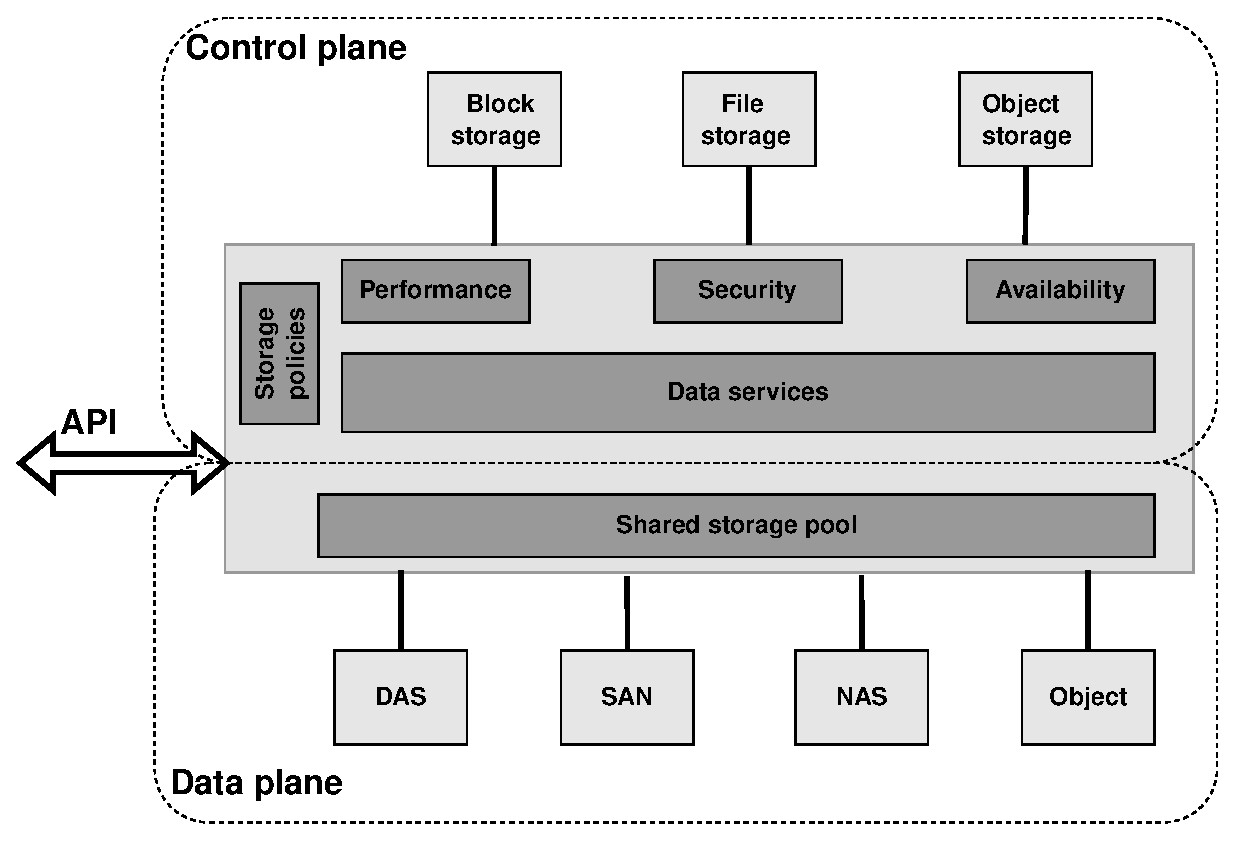
\includegraphics[width=1\textwidth]{obrazky-figures/sds-planes.eps}
        \caption{SDS data and control plane (source: \cite{sdsPlanes}, remade).}
        \label{fig:sdsPlanes}
    \end{figure}

\section{Beanstalk queue}

    Beanstalk queue or shorter \textbf{beanstalkd} is a fast, simple and lightweight working queue\cite{beanstalkdOfficial}. The primary use case is to manage workflow between different parts of workers of application through working queues and messages. Beanstalkd was developed for the need of Facebook application in order to reduce average response time\cite{beanstalkdOfficial}. Provided by simple protocol design, heavily inspired by Memcached, implemented in programming language C, Beanstalkd offers lean architecture, which allows it to be installed and used very simply, making it perfect for many use cases\cite{beanstalkdInstall}.


    \subsection{Beanstalkd elements}
    Beanstalkd is a priority queue with server-client architecture. The server represents queues where jobs are saved based on priority. Beanstalkd architecture is composed of several components:
    \begin{itemize}
        \item \textbf{Jobs} - tasks stored by the client
        \item \textbf{Tubes} - used for storing tasks, each tube contains a ready queue and a delay queue.
        \item \textbf{Producer} - creates and sends jobs to beanstalkd using command \texttt{put}.
        \item \textbf{Consumer} - process "listening" on an assigned tube, reserves and consumes jobs from the tube.
    \end{itemize}

    \subsection{Job Lifecycle}
    Each job is uniquely assigned to one worker at a time. The client creates a job and inserts it into a beanstalkd tube using the \texttt{put} command. While being in the tube, the job can be in next states\cite{beanstalkdProtocol}:
    \begin{itemize}
        \item \texttt{\textbf{Ready}} - the task is free and can be executed immediately by the Consumer.
        \item \texttt{\textbf{Delayed}} - the task has assigned delay time that needs to expire before execution. After delay time expires, beanstalkd will automatically change its state to \texttt{Ready}.
        \item \texttt{\textbf{Reserved}} - the task is reserved and is being executed by the \textit{Consumer}. Beanstalkd is responsible for checking whether the task is completed in time (\textbf{TTR} - Time to run).
        \item \texttt{\textbf{Buried}} - reserved task, the task will not be removed nor executed until the client decides. This state is often used for further inspection in debugging process when failure or undefined behavior occurs during task execution.
        \item \texttt{\textbf{Deleted}} - the task is deleted from the tube, beanstalkd no longer maintains these jobs.
    \end{itemize}

    Figure \ref{fig:beanstalkdJobSM} describes the life cycle of a job in a beanstalkd tube. Job is created by \textit{Producer} using put command. Beanstalkd allows the \textit{Producer} to add delay time before the task is ready for execution, setting the job state to \texttt{Delayed}. After delay time expires, beanstalkd will automatically change job state to \texttt{Ready}. The Producer can specify job priority and jobs with the \texttt{Ready} state are stored in the priority queue. A job with the biggest priority is reserved and executed by a \textit{Consumer}. After successfully executing the task, the \textit{Consumer} will delete the job from beanstalkd. If some error occurs, the \textit{Consumer} can \textbf{bury} the task. The Consumer can decide that he is not interested in completing the reserved task. Using the \texttt{release} command (with optional delay) job state will be changed back to \texttt{Ready} (or \texttt{Delay} if delay exists). Jobs with the \texttt{Burried} state will not be touched by the beanstalkd server until the client \texttt{"kicks"} them to \texttt{READY} state.

    \begin{figure}[H]
        \centering
        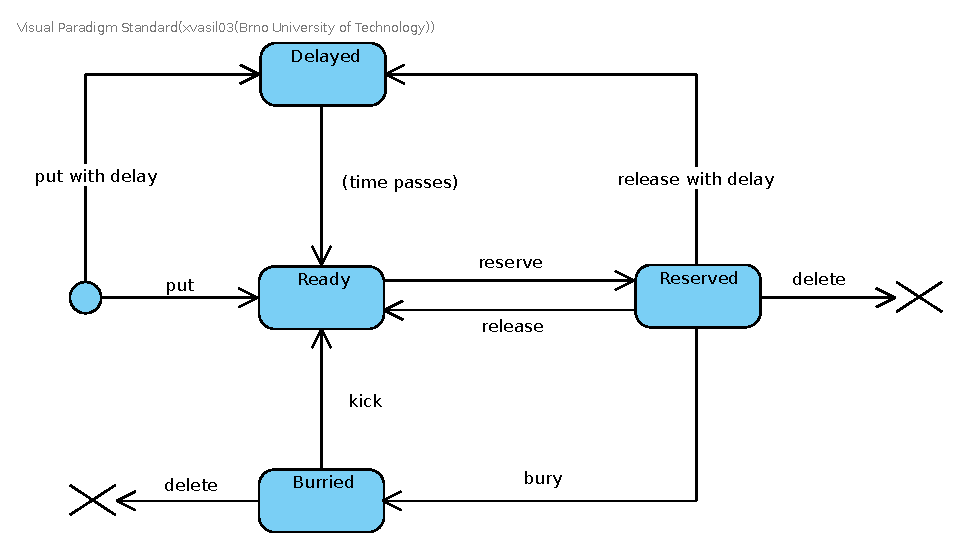
\includegraphics[width=1\textwidth]{obrazky-figures/beanstalkd-job-states.eps}
        \caption{State machine diagram of job in Beanstalkd tube.}
        \label{fig:beanstalkdJobSM}
    \end{figure}


    \subsection{Key characteristics}
    Key beanstalkd characteristics are:

    \paragraph{Asynchronous}- beanstalkd allows producers to put jobs in the queue, and workers can process them later.
    \paragraph{Distributed}- in the same way as \textit{Memcached}\footnote{Memcached - in-memory key-value store {\url{https://memcached.org/}}}, beanstalkd can be distributed, although this distribution is handled by clients. The beanstalkd server does not know anything about other beanstalkd running instances.
    \paragraph{Persistent}- beanstalkd offers support for persistent jobs during which all jobs are written to binlog. In case of a power outage, after restarting a beanstalkd instance, it will recover jobs content from the logs.
    \paragraph{Not secured}- beanstalkd is designed to be run in a private/secure network. Therefore it \textbf{does not support authentication or authorization}.
    \paragraph{Scalability}- beanstalkd can be scaled horizontally, although it must be done on the client side, where each client would connect to multiple servers and then use specific algorithms(e.g., Round-robin) to switch between the different servers.

\section{Event notifications}
    %introduction
     \textbf{An event} is a runtime operation executed by a software element, representing a significant change or occurrence in a system. Event is created in order to make some information available to other software elements not specified by the operation\cite{eventArchitecturalPatterns}.

    \textbf{Event notification} is a message created by a system in order to notify other parts of the system that an event has taken place\cite{eventRedHatEventDrivenArch}. Event notifications are usually used for monitoring and asynchronous job processing.

    In object storage, event notifications are used to notify users or tenants about specific changes and occurrences in their bucket or account. Typical event notifications include creating new (or updating existing) objects in the bucket. In addition, most object vendors offer \textbf{publish/subscribe} notifications, allowing users to subscribe to certain types of event notifications using predefined rules. Information about rules specifying event notifications is usually stored in the upper-level metadata (bucket or account).

    \subsection{CloudEvents}
    Publishers tend to describe event data differently due to non-existing standards or formats. The lack of a common way to describe events means developers have to learn how to handle events from each event source. To solve this problem, CloudEvents was created.

    \textbf{CloudEvents} is a specification for describing event data in common way\cite{eventCloudEvents} hosted by CNCF\footnote{CNCF - Cloud Native Computing Foundation {\url{https://www.cncf.io/}}}. CloudEvents goal is to dramatically simplify event specification and delivery across services, platforms and beyond.
    CloudEvents has been integrated by many popular object storage vendors, such as Oracle Cloud, IBM Cloud Code Engine, Azure, Google Cloud, etc.

    Attributes in CloudEvents specification can be divided into three categories:
    \paragraph{Required attributes} - set of attibures that are required to be included in all events\cite{eventCloudEventsSpec}:
    \begin{itemize}
        \item id (string) - event identifier, must not be empty.
        \item source (URI-reference) - identifies context in which event occured, must not be empty.
        \item specversion (string) - the version of CloudEvents specification, must not be empty.
        \item type (string) - value describing the type of occurred event. Often this attribute is used for policy enforcement, routing and monitoring.
    \end{itemize}

    \paragraph{Event data attirbutes} - attibures containing and describing event data:
    \begin{itemize}
        \item datacontenttype (string) - content type of data value (allows data to carry any type of content).
        \item dataschema (URI) - identifies the schema that data adheres to.
        \item data - data payload
    \end{itemize}

    \paragraph{Optional attributes}:
    \begin{itemize}
        \item time - timestamp
        \item subject (string) - the subject of the event in the context of the event producer.
        \item extension attributes - custom attibutes allowing external systems to attach metadata to an event.
    \end{itemize}

    \begin{lstlisting}[style=jsonStyle, caption=Example of event described using CloudEvents specification in JSON format.]
    {
        "specversion" : "1.0",
        "type" : "com.github.pull_request.opened",
        "source" : "https://github.com/cloudevents/spec/pull",
        "subject" : "123",
        "id" : "A234-1234-1234",
        "time" : "2018-04-05T17:31:00Z",
        "comexampleextension1" : "value",
        "comexampleothervalue" : 5,
        "datacontenttype" : "text/xml",
        "data" : "<much wow=\"xml\"/>"
    }
    \end{lstlisting}

    \subsection{Amazon S3 event notifications}
    \textbf{Amazon Simple Storage Service (S3)} is one of the most popular cloud object storages providing a \texttt{REST} web service interface. Amazon S3 is reliable, scalable, commercial and one of the most popular object storage that manages Web-Scale computing by itself\cite{eventS3}. As a result, Amazon S3 has a big impact on object storage and most other object storage vendors crated compatible \textbf{S3 API} for their services.

    One of the monitoring features that Amazon S3 provides is \textbf{Event Notification}, which offers users to receive notifications when certain events happen in their S3 bucket. To enable such notifications, users need to create a notification configuration that identifies which events Amazon S3 should publish\cite{eventS3EventNotification}. Notifications are configured at the bucket level and then applied to each object in the bucket.

    Amazon S3 provides limited event destinations to which event notification messages can be send\cite{eventS3EventNotificationDest}:
    \begin{itemize}
        \item \textit{Amazon Simple Notification Service (Amazon SNS)} - flexible, fully managed push messaging service, can be used to send messages to mobile phones or distributed services.
        \item \textit{Amazon Simple Queue Service (Amazon SQS)} queues - reliable and scalable hosted queues for storing messages as they travel between computers.
        \item \textit{AWS Lambda} - serverless, event-driven compute service. Lambda can run custom code in response to the Amazon S3 bucket event (if the lambda function writes to the same bucket that triggers the notification, it can create an execution loop).
        \item \textit{Amazon EventBridge} - serverless event bus service used to receive events from AWS. It allows users to define rules to match events and deliver them to defined targets.
    \end{itemize}

    By this date, Amazon S3 \textbf{does not support CloudEvents} specification and describes event data in its own way. Some of the event types that Amazon S3 can publish are displayed in table \ref{tab:eventTypesS3}.


     \renewcommand*{\arraystretch}{1.4}
     \begin{table}[H]
     \begin{tabularx}{\textwidth}{|p{0.3\textwidth}|X|}
         \hline
         \textbf{Event type} & \textbf{Desription} \\
         \hline
         s3:TestEvent & after enabling the event notifications, Amazon S3 publishes a test notification to ensure that topic exist and bucket owner has permissions to publish specified topic. \\
         \hline
         s3:ObjectCreated:* & An object was created (regardless on operation). \\
         \hline
         s3:ObjectCreated:Put & An object was created by an HTTP PUT operation. \\
         \hline
         s3:ObjectCreated:Post & An object was created by HTTP POST operation. \\
         \hline
         s3:ObjectCreated:Copy & An object was created an S3 copy operation. \\
         \hline
         s3:ObjectCreated:

         CompleteMultipartUpload & An object was created by the completion of a S3 multi-part upload. \\
         \hline
         s3:ObjectRemoved:* & An object was removed (regardless on operation). \\
         \hline
         s3:ObjectRemoved:Delete & An object was deleted by HTTP DELETE operation. \\
         \hline
         s3:ObjectRemoved:

         DeleteMarkerCreated & An versioned object was marked for deletion. \\
         \hline
    \end{tabularx}
    \caption{Subset of Amazon S3 Event Types \cite{eventS3EventNotificationDest}\label{tab:eventTypesS3}}
    \end{table}

\chapter{Object storages}\label{chap:object-storages}
    \section{OpenIO SDS}
    This section introduces OpenIO Software-defined storage, its key features, its data organization along with the underlying technologies. Furthermore, this section introduces Grid For Apps framework (\ref{sec:oioGridForApps}) and event publishing in OpenIO (\ref{sec:oioEvent-Agent}).

    OpenIO Software-defined storage is open source object storage that is perfectly capable of traditional use cases (such as archiving, big data, cloud). However, at the same time, combined with Grid for Apps (\ref{sec:oioGridForApps}), it opens the door for users to create an application that needs much more sophisticated back-end operations. These applications include industrial IoT, machine learning and artificial intelligence, as well as any other applications whose workflow can benefit from automated jobs or tasks\cite{oioNextGen}. In addition, OpenIO SDS is event-driven storage with the ability to intercept events seamlessly and transparently to the rest of the stack.

    \subsection{Key characteristics}
    \paragraph{Hardware agnostic}
    OpenIO SDS is fully software-defined storage capable of running on x86 or ARM hardware with minimal requirements. Cluster nodes can be different from each other, allowing different generations, types, and capacities to be combined without affecting a performance or efficiency\cite{oioKeyChars}.
    OpenIO has built-in support for heterogeneous hardware allowing every node to be used at its maximum performance.
    \paragraph{No SPOF architecture}
    Every single service used to serve data is redundant from object chunks stored in a disc to the directory level, every information is duplicated. As a result, there is no single point of failure (SPOF) in the cluster and a node can be shut down without affecting overall availability or integrity\cite{oioCoreSolution}.
    \paragraph{Cluster organization}
    Instead of a traditional cluster ring-like layout, OpenIO SDS is based on a grid of nodes \ref{fig:oioArch}. It is flexible and resource-conscious. Compared to other object storage solutions, cluster organization is not based on static data allocation that usually use Chord peer-to-peer distributed hash table algorithm. Instead, OpenIO SDS uses distributed directory for organizing data and metadata hash tables, which allows the software to attain the same level of scalability but with better and more consistent performance\cite{oioKeyChars}.

    \begin{figure}[H]
        \centering
        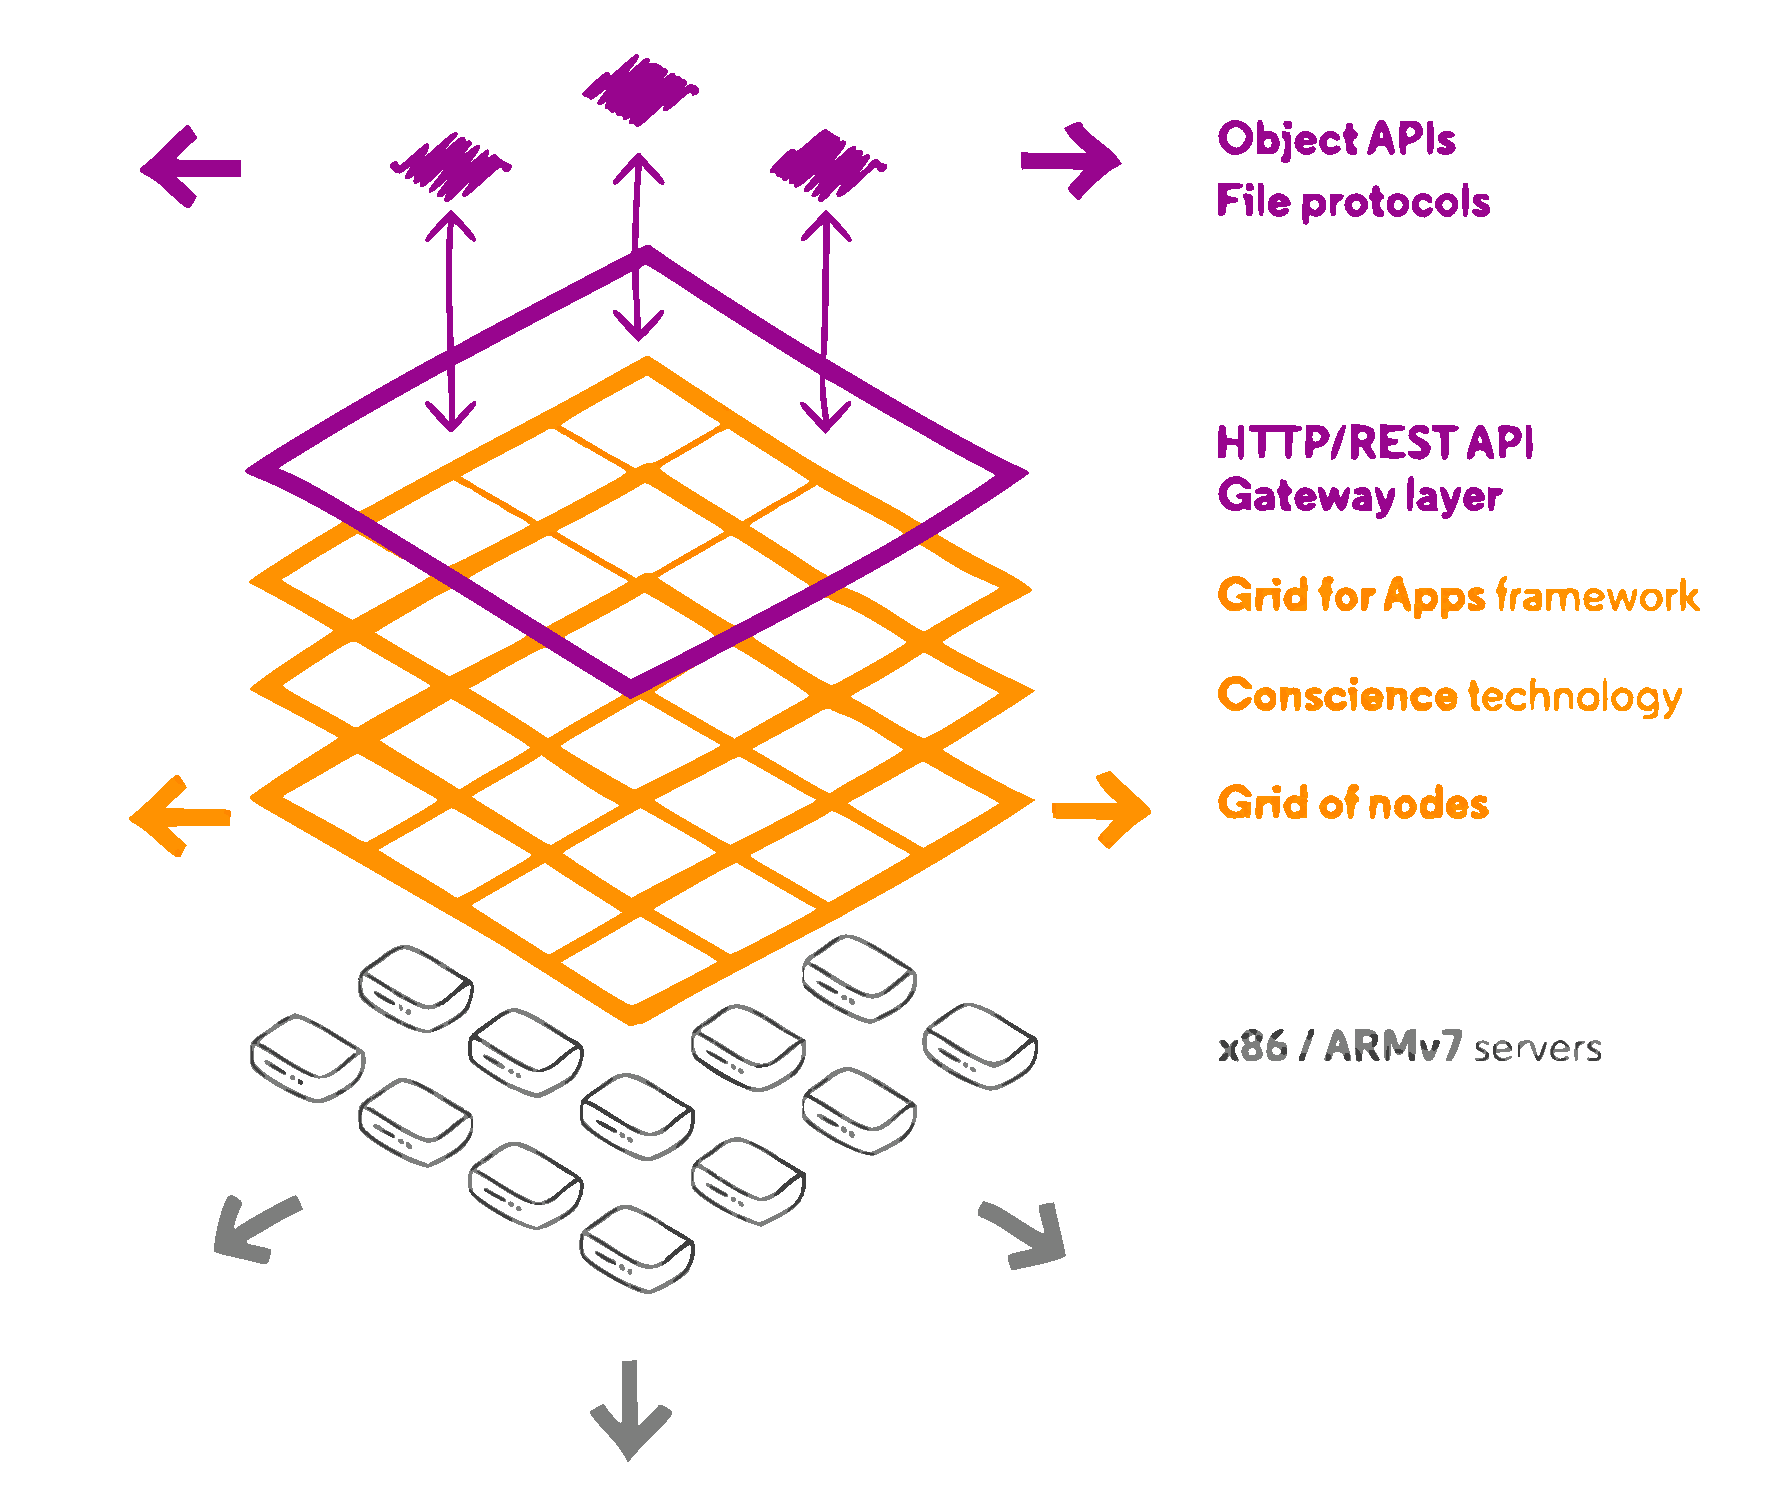
\includegraphics[width=1\textwidth]{obrazky-figures/openio-architecture.eps}
        \caption{Layered view on OpenIO SDS architecture (source: \cite{oioArch}).}
        \label{fig:oioArch}
    \end{figure}


    \paragraph{Tiering}
    With tiering, OpenIO SDS offers users to configure a pool containing a group of hardware that can then be used to store specific types of objects. For example, users can create a pool of high-performance hard disks (e.g. SSDs) and use the pool to store objects that require low latency.
    This feature is realized by a mechanism called \textbf{storage policies}. Multiple storage policies can be defined in one particular namespace. Storage policies can also be used for specifying how many replicas should be created for a specific dataset\cite{oioCoreSolution}.

    \paragraph{ConsciousGrid}
    ConsciousGrid is an OpenIO technology that uses real-time metrics from the nodes(CPU, I/O, capacity) automatically discover and place data in the most appropriate place. It provides \textbf{load balancing} and computes a score for each node and then provides weighted random selection\cite{oioSdsServices}.


    \subsection{Data organization}
    Multi-tenancy is one of the core concepts in OpenIO SDS. Data objects are stored within following hierarchy: \texttt{Namespace/Account/Container/Object} \ref{fig:oioDataOrganization}. Multiple namespaces can be configured in each cluster, providing multi-region/zone logical layouts for applications and segregated workloads depending on a tenant or geo-distribution need\cite{oioSdsConcepts}.
    There is no classic subdirectory tree. Instead, objects are stored in a flat structure in the container level. However, like many other object storages, there is a way to emulate a filesystem.

    \begin{figure}[H]
        \centering
        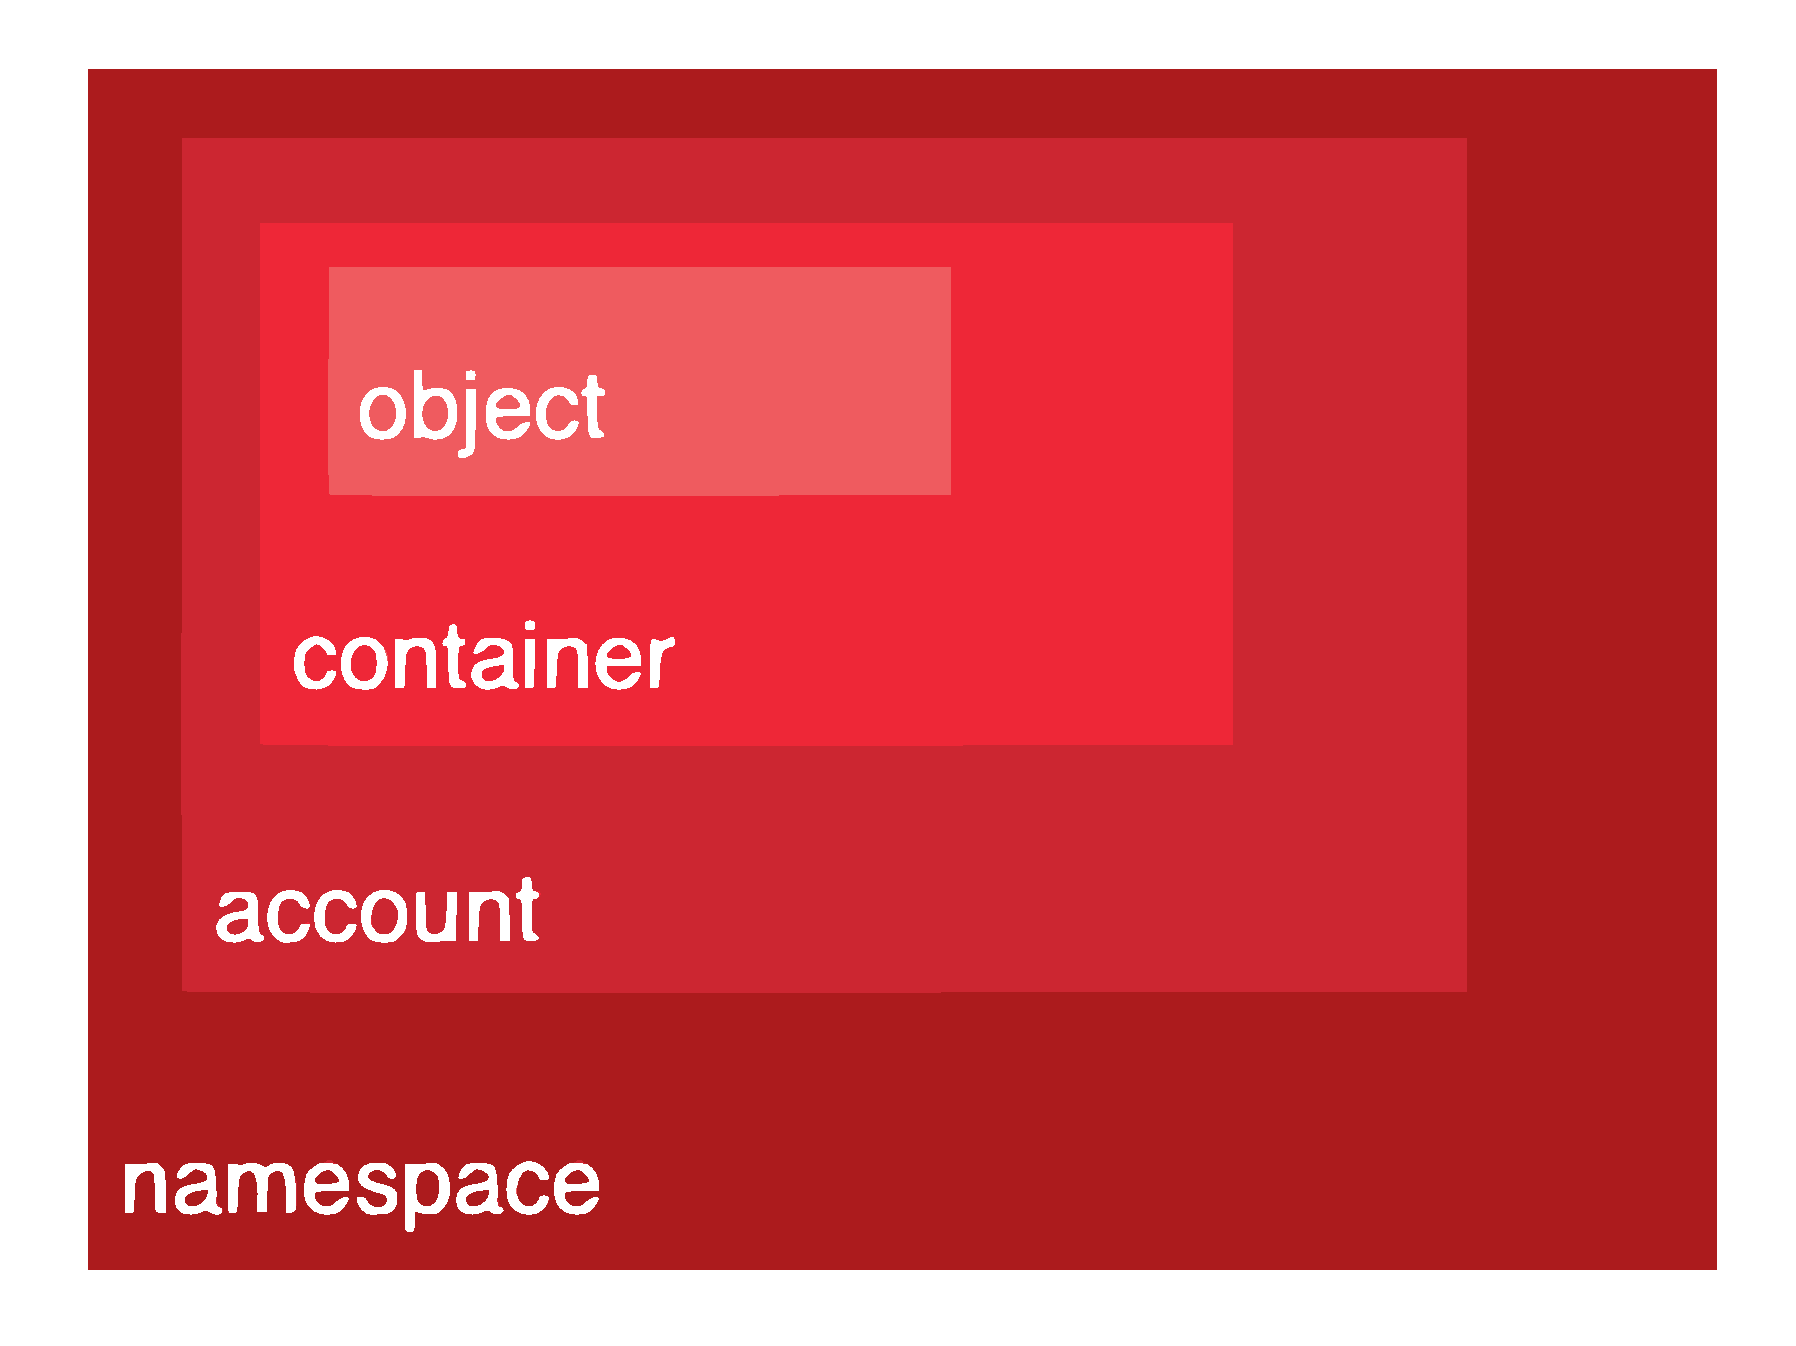
\includegraphics[width=0.5\textwidth]{obrazky-figures/openio-data-organization.eps}
        \caption{Object data organization in OpenIO SDS (source: \cite{oioCoreSolution}).}
        \label{fig:oioDataOrganization}
    \end{figure}

    \paragraph{Namespace}
    A coherent set of network services working together to run OpenIO's solutions. It hosts services and provides operations such as service configuration and monitoring.

    \paragraph{Account}
    An account usually represents a tenant and is the top level of data organization. Each account owns and manages a collection of containers. In addition, the account keeps track of namespace usage for each customer (i.e. bytes occupied by all of a customer's objects)\cite{oioCoreSolution}.

    \paragraph{Container}
    Container represents an object bucket. Each container belongs to one (and only one) account and is identified by a unique name within the account. The container carries additional information specifying how to manage its objects (e.g. how to secure them)\cite{oioCoreSolution}.

    \paragraph{Object}
    Object is the smallest data unit visible by a customer and represents a named BLOB with metadata. OpenIO SDS allows several objects to be stored in a container and are considered versions of the same object. Classic \texttt{API} operations (\texttt{PUT/GET/DELETE}) will be directed towards an object with the latest version. If the size of an object is larger than the specified limit at the namespace level, the object will be divided into chunks of data. This behavior allows capacity optimization as well as \textbf{distributed reads} that could be particularly useful for high-speed video streaming of large media\cite{oioCoreSolution}.

    %todo authentication and acl?

    %\section{Services} maybe include?
    \subsection{Serverless computing}
    OpenIO offers Serverless computing in object storage cluster nodes using the framework Grid For Apps.
    \paragraph{Grid For Apps}\label{sec:oioGridForApps}

    Like Amazon AWS Lambda, OpenIO offers an \textbf{event-driven compute service} called Grid for Apps that works on top of OpenIO.

    Grid for Apps intercepts all the events that happen in the storage layer, and based on user configuration, triggers specific applications or scripts to act on data (metadata) stored in object storage\cite{oioNextGen}. The application is executed in cluster nodes and utilizes free unused resources available in the cluster. This improves efficiency (fewer data moving since object data are already available) and saves money (no need for external resources)\cite{oioNextGen}.

    Grid for Apps allows customers to perform operations such as metadata enrichment, data indexing and search (e.g. indexing metadata to Elasticsearch), pattern recognition, machine learning, data filtering, monitoring, etc\cite{oioNextGen}.

    Grid for Apps in OpenIO is realized using service \texttt{event-agent} and \texttt{beanstalkd} queue.

    \paragraph{Event-agent}\label{sec:oioEvent-Agent}
    Event-agent is an OpenIO service responsible for handling asynchronous jobs. It relies on beanstalkd backend to manage jobs. Event-agent key characteristics are\cite{oioSdsServices}:
    \begin{itemize}
        \item Stateless
        \item CPU intensive
        \item Must be deployed on every server of the cluster
    \end{itemize}

    Every event that occurs in OpenIO is inserted in a beanstalkd tube. Event-agent is listening to the beanstalkd tube and consumes jobs from it. Consumers are produced using Eventlet Network Library \cite{oioEventlet}. The number of workers can be configured.

    In event-agent, users can specify handlers for each type of event in event-handler.conf.
    Some of the event types in OpenIO are \texttt{storage.content.new} (e.g., new object in storage), \texttt{storage.container.deleted} (e.g., object has been deleted), etc.

    \textbf{Events handler} is defined as a pipeline containing applications that will react to the event. In example \ref{lst:event-agent-handlers}, deleting an object will invoke \texttt{storage.content.deleted} event. Event-agent will handle the event using \texttt{content\_cleaner} application, which deletes objects chunks from object storage.

    OpenIO offers users to process events outside of the event-agent. In order to do that, users can use the application \texttt{notify} which will send an event to a specified beanstalkd tube. Then a user can create a custom consumer process that will execute the job from beanstalkd tube. An example of such configuration is displayed in listing \ref{lst:event-agent-handlers}.

    \lstset{
        caption=Example of event-agent handler configuration,
        label=lst:event-agent-handlers
    }
    \begin{minipage}{\linewidth}
    \begin{lstlisting}
    [handler:storage.content.deleted]
    pipeline = content_cleaner

    [handler:storage.content.new]
    pipeline = notify

    [filter:content_cleaner]
    use = egg:oio#content_cleaner

    [filter:notify]
    use = egg:oio#notify
    tube = oio-rebuild
    queue_url = ${QUEUE_URL}
    \end{lstlisting}
    \end{minipage}

    \subsection{OIO-Swift}
    One of the key components in OpenIO SDS system is OIO-Swift service, which acts like gateway. Main responsibility of this component is to handle Swift/S3 user requests. Implementation of OIO-Swift is based on OpenStack Swift Proxy server. OIO-Swift key features include:
    \begin{itemize}
        \item Operations on objects, containers and accounts.
        \item Authentication support (using OpenStack Keystone).
        \item Metadata support - enables usage of system metadata.
        \item Swift Middleware support - allow running Swift middlewares within OpenIO SDS system.
    \end{itemize}

\newpage
\section{OpenStack Swift}
    This section introduces OpenStack object storage (code name Swift) and describes its key features. Furthermore, this section elaborates OpenStack Swift architecture, introduces its main services and interfaces for communication with object storage.

    OpenStack Swift is open-source object storage developed by Rackspace, a company that, together with NASA, created the OpenStack project. After becoming an open-source project, Swift became the leading open-source object storage supported and developed by many famous IT companies, such as Red Hat, HP, Intel, IBM, and others.

    OpenStack Swift is a multi-tenant, scalable, and durable object storage capable of storing large amounts of unstructured data at low cost\cite{swiftOpenStackSwift}.

    \subsection{Key characteristics}
    Besides standard object storage characteristics (like scalability, durability, hardware agnostic, etc.), some of the keys OpenStack Swift characteristics:

    \paragraph{Multi-regional capability}
    OpenStack Swift has distributed architecture. Data can be distributed and replicated into multiple data centers, although the negative effect could be higher latency between them. Distribution can provide high availability of data and recovery site\cite{swiftOpenStackSwift}.

    \paragraph{No SPOF}
    With all data being replicated and distributed, there is no single proof of failure in OpenStack Swift architecture.

    \paragraph{Developer-friendliness}
    OpenStack Swift offers many built-in features that developers and users can use. some of the most interesting built-in features are\cite{swiftOpenStackSwift}:
    \begin{itemize}
        \item \textbf{Automatically expiring objects} - Objects can be given expiration time, after which objects become invalid and deleted from object storage.
        \item \textbf{Quotas} - Storage limits can be configurated on container/account level.
        \item \textbf{Versioned objects} - User can store a new version of an object, while object storage keeps previous (older) versions.
        \item \textbf{Access control lists} - Users can configure access to their data to give or deny permission for reading or writing data to other users.
    \end{itemize}

    \paragraph{Middleware support}
    - OpenStack Swift allows adding custom middlewares, which will be run directly on storage system\cite{swiftEssentials}. This feature can be used for monitoring purposes, for example, informing users or other applications about new objects in storage using Webhook middleware.

    \paragraph{Large object support}
    - By default, OpenStack Swift has a limit on a single uploaded object, which is 5GB. However, using segmentation, the size of a single object can be virtually unlimited. This option offers a possible higher upload speed, in case of parallel upload\cite{swiftLOS}.

    \paragraph{Partial object retrival}
    Users can retrieve part of an object, for example, just a portion of a movie object file\cite{swiftImplementingCloudStorage}.

    \subsection{Data model}
    OpenStack Swift allows users to store unstructured data objects with a canonical name containing \textit{account}, \textit{container} and \textit{object} in given order\cite{swiftOpenStackSwift}. The account names must be unique in the cluster, the container name must be unique in the account space, and the object names must be unique in the container. Other than that, if containers have the same name but belong to a different account, then they represent different storage locations. The same principle applies to objects. If objects have the same name but not the same container and account name, then these objects are different.

    \paragraph{Account}
    Accounts are root storage locations for data. Each account contains a list of containers within the account and metadata stored as key-value pairs. Accounts are stored in the account database. In OpenStack Swift, account is \textbf{storage account} (more like storage location) and \textbf{do not represent a user identity}\cite{swiftOpenStackSwift}.

    \paragraph{Container}
    Containers are user-defined storage locations in the account namespace where objects are stored. Containers are one level below accounts, therefore they are not unique in the cluster. Each container has a list of objects within the container and metadata stored as key-value pairs. Containers are stored in container database\cite{swiftOpenStackSwift}.

    \paragraph{Object}
    An object represents data stored in OpenStack Swift. Each object belongs to one (and only one) container. An object can have metadata stored as key-value pairs. Swift stores multiple copies of an object across the cluster to ensure durability and availability. Swift does this by assigning an object to \textit{partition}, which is mapped to multiple drives, and each driver will contain object copy\cite{swiftOpenStackSwift}.

    \paragraph{Server Processes}
    The path towards data in OpenStack Swift consists of four main software services: \textbf{Proxy server}, \textbf{Account server}, \textbf{Continaer server} and \textbf{Object server}. Typically Account, Container and Object server are located on same machine creating \textbf{Storage node}.

    \paragraph{Proxy server}
    The proxy server is the service responsible for communication with external clients. For each request, it will look up storage location(node) for an account, container, or object and route the request accordingly\cite{SwiftArchitecturalOverview}. The proxy server is responsible for handling many failures. For example, when a client sends a \texttt{PUT} request to OpenStack Swift, the proxy server will determine which nodes store the object. If some node fails, a proxy server will choose a hand-off node to write data. When a majority of nodes respond successfully, then the server proxy will return a success response code\cite{swiftOpenStackSwift}.

    \paragraph{Account server}
    Account server stores information about containers in a particular account to SQL database. It is responsible for listing containers. It does not know where specific containers are, just what containers are in an account\cite{SwiftArchitecturalOverview}.

    \paragraph{Container server}
    Container server is similar to account server, except it is responsible for listing objects and also does not know where specific objects are\cite{SwiftArchitecturalOverview}.

    \paragraph{Object server}
    The Object Server is blob storage capable of storing, retrieving, and deleting objects. Objects are stored as binary files to a filesystem, where metadata are stored in the \textit{file's extended attributes (xattrs)}. This requires a filesystem with support of such attributes. Each object is stored using a hash value of object path (account/container/object) and timestamp. This allows storing multiple versions of an object. Since last write wins (due to timestamp), it is ensured that the correct object version is served\cite{SwiftArchitecturalOverview}.

    \begin{figure}[H]
        \centering
        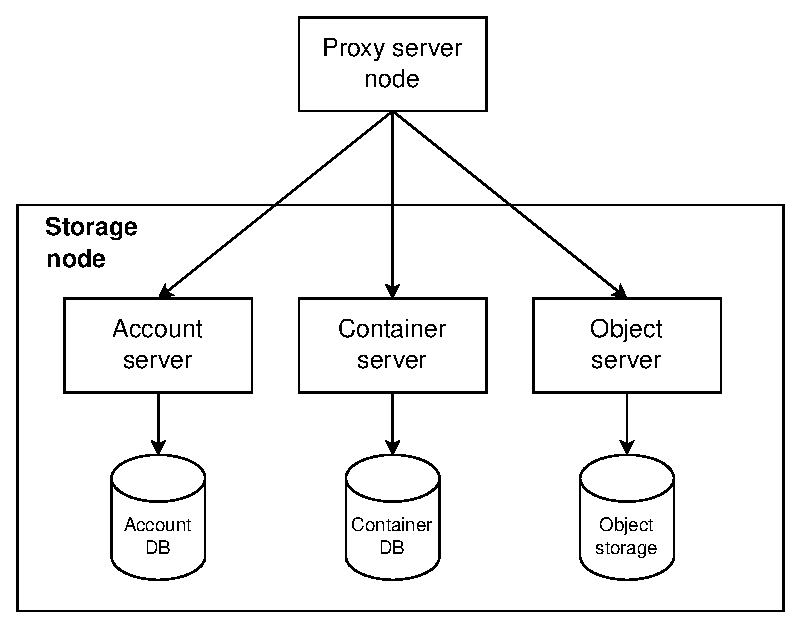
\includegraphics[width=0.75\textwidth]{obrazky-figures/swift-servers.eps}
        \caption{OpenStack Swift servers architecture.}
        \label{fig:swiftServers}
    \end{figure}

    \subsection{Middlewares}
    Using Python WSGI middleware, users can add functionalities and behaviors to OpenStack Swift. Most middlewares are added to the Proxy server but can also be part of other servers (account server, container server, or object server).

    Middlewares are added by changing the configuration of servers. In example \ref{lst:swiftMiddleware}
    \texttt{webhook middleware} is added into the proxy server by changing its pipeline (\textit{pipeline:main}). Middlewares are executed in the given order (first will be called webhook middleware, then proxy-server middleware).

    Some of the middlewares are required and will be automatically inserted by swift code\cite{swiftMiddleware}.

    \lstset{
        caption=Example of proxy server configuration (proxy-server.conf).,
        label=lst:swiftMiddleware
    }
    \begin{lstlisting}
    [DEFAULT]
    log_level = DEBUG
    user = <your-user-name>

    [pipeline:main]
    pipeline = webhook proxy-server

    [filter:webhook]
    use = egg:swift#webhook

    [app:proxy-server]
    use = egg:swift#proxy
    \end{lstlisting}

    \paragraph{Interface}
    OpenStack Swift servers are implemented using Python WSGI applications. Therefore only Python WSGI middlewares are accepted in OpenStack Swift.

    In listing \ref{lst:swift-healthcheck} is example of simplified \texttt{healthcheck middleware}. The constructor takes two arguments, the first is a WSGI application, and the second is a configuration of middleware defined using Python Paste framework in \texttt{proxy-server.conf}. Middleware must have a call method containing the request environment information and response from previously called middleware. Middleware can perform some operations and call the next middleware in the pipeline or intercept a request. In the healtcheck example, if the path directs to \texttt{/healtcheck} , the middleware will return \texttt{HTTP Response}, and other middlewares in the pipeline will not be called.

    Method \texttt{filter\_factory} is used by the Python Paste framework to instantiate middleware.

\begin{lstlisting}[language=Python, style=pythonStyle, caption=Example of healthcheck middleware in OpenStack Swift, label=lst:swift-healthcheck]
import os
from swift.common.swob import Request, Response

class HealthCheckMiddleware(object):
    def __init__(self, app, conf):
        self.app = app

    def __call__(self, env, start_response):
        req = Request(env)
        if req.path == '/healthcheck':
            return Response(request=req, body=b"OK", content_type="text/plain")(env, start_response)
        return self.app(env, start_response)

def filter_factory(global_conf, **local_conf):
    conf = global_conf.copy()
    conf.update(local_conf)

    def healthcheck_filter(app):
        return HealthCheckMiddleware(app, conf)
    return healthcheck_filter
\end{lstlisting}

    \paragraph{Metadata}
    OpenStack Swift separates metadata into 3 categories based on their use:
    \begin{itemize}
        \item \textbf{\texttt{User Metadata}} - User metadata takes form \texttt{X-<type>-Meta-<key>: <value>}, where \texttt{<type>} represent resource type(i.e. account, container, object), and \texttt{<key>} and \texttt{<value>} are set by user. User metadata remain persistent until are updated using new value or removed using header \texttt{X-<type>-Meta-<key>} with no value or a header \texttt{X-Remove-<type>-Meta-<key>: <ignored-value>}.
        \item \textbf{\texttt{System Metadata}} - System metadata takes the form of \texttt{X-<type>-Sysmeta-<key>: <value>}, where \texttt{<type>} represent resource type(i.e. account, container, object) and \texttt{<key>} and \texttt{<value>} are set by internal service in Swift WSGI Server.
        All headers containing system metadata are deleted from a client request.

        System metadata are visible only inside Swift, providing a means to store potentially sensitive information regarding Swift resources.
        \item \textbf{\texttt{Object Transient-Sysmeta}} - System metadata takes the form of \texttt{\newline X-Object-Transient-Sysmeta-<key>:<value>}. Transient-sysmeta has a similar behavior as system metadata and can be accessed only within Swift, and headers containing Transient-sysmeta are dropped. If middleware wants to store object metadata, it should use transient-sysmeta\cite{swiftMiddleware}.
    \end{itemize}

\newpage
\section{MinIO}\label{chap:minio}
This section introduces MinIO object storage, describes its key features, most essential components, and event notifications in MinIO.

    \subsection{Introduction}
    MinIO is software-defined object storage that provides high performance and scalability. MinIO was designed to be the standard in private/hybrid cloud object storage.
    It runs on industry-standard hardware and is 100\% open source\cite{minioObjectStorage}.

    MinIO software-defined object storage suite consists of a \textit{MinIO server} and optional components.

    \paragraph{MinIO Server} - MinIO Server is distributed object storage server.
    \paragraph{MinIO Client} - Service provoding familiar UNIX commands like \textit{ls, cat, cp, diff} in MinIO storage.
    \paragraph{MinIO Console} - Browser-based GUI offering all commands from MinIO Client in a design that feels more intuitive for DevOps and IT admins.
    \paragraph{MinIO Kubernetes Operator} - plugin allowing easy deployment and operation of MinIO object storage on Kubernetes.

    \subsection{Key features}
    MinIO was designed to multiple benefits to object storage:

    \paragraph{Ease of use}
    MinIO can be installed simply by downloading a single binary file and executing it. The configuration setup has been kept to a bare minimum. Upgrading to a newer version is done with a single command, which is non-disruptive and does not provoke any downtime\cite{minioIntel}.

    \paragraph{Encryption and WORM}
    MinIO provides per-object encryption using a unique object key protected by a master key managed key-management system (KMS).

    MinIO supports object locking by enforcing \textit{Write-Once-Read-Many(WORM)} immutability until the lock is expired or lifted. This mode prevents tempering with data once written\cite{minioHighPerformance}.

    \paragraph{Metadata architecture}
    MinIO does not provide separate storage for metadata. All operations are performed on object-level granularity. This approach isolates any failures and does not allow any spillover to larger system failures\cite{minioIntel}.

    \paragraph{High availability}
    MinIO design allows a server to lose up to half its drivers and a cluster to lose up to half its servers, and MinIO will still be able to successfully process requests and serve objects. This is achieved by erasure code that protects data with redundancy\cite{minioIntel}.

    \subsection{Architecture}
    MinIO is designed to be cloud-native object storage to be run in lightweight containers managed by external orchestration service such as Kubernetes. The entire server is ~40MB static binary and is highly effective in its use of CPU and memory resources. This allows co-hosting multiple numbers of tenants on shared hardware\cite{minioObjectStorage}.

    Usually, storages are built using multi-layer storage architecture, with a durable block layer at the bottom, a virtual file system in the middle layer, and multiple API gateways providing multiple protocols for emulating file, block, and object manipulation. The problem with this approach is that it has too many compromises\cite{minioIntel}.

    MinIO decided on a completely different approach compared to other storage systems. Since MinIO's primary purpose is to serve only objects, it was built using \textbf{single-layer architecture} that provides all necessary functionalities without compromises. The advantage of this approach is object storage with high performance and lightweight\cite{minioIntel}.

    In MinIO single-layer architecture, there is no such thing as Metadata server, but objects \textit{data and metadata are stored together}, which eliminates the need for a metadata database. In addition, MinIO performs all functions (erasure code, bitrot check, encryption) as inline, strictly consistent operations. This metadata design allows, in case of damage of an object, the damage can be healed/corrected for the individual object\cite{minioHighPerformance}.

    Figure \ref{fig:minio-architecture} visualize MinIO cluster architecture. Each MinIO cluster is a collection of distributed MinIO servers attached to local drivers (JBOD/JBOF). Drivers are grouped into erasure sets and objects are stored into these sets using a hashing algorithm\cite{minioObjectStorage}.

    \begin{figure}[H]
        \centering
        %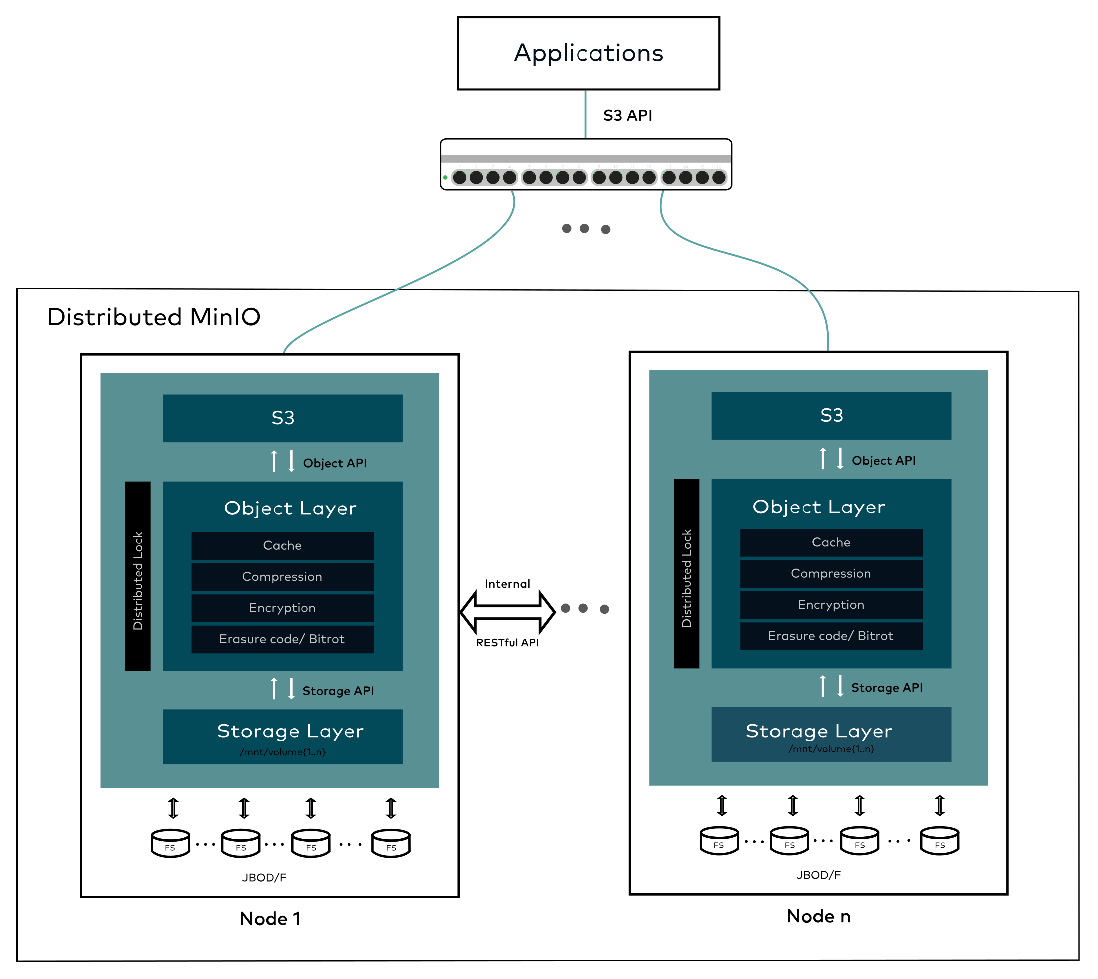
\includegraphics[width=0.8\textwidth]{obrazky-figures/minio-architecture.eps}
        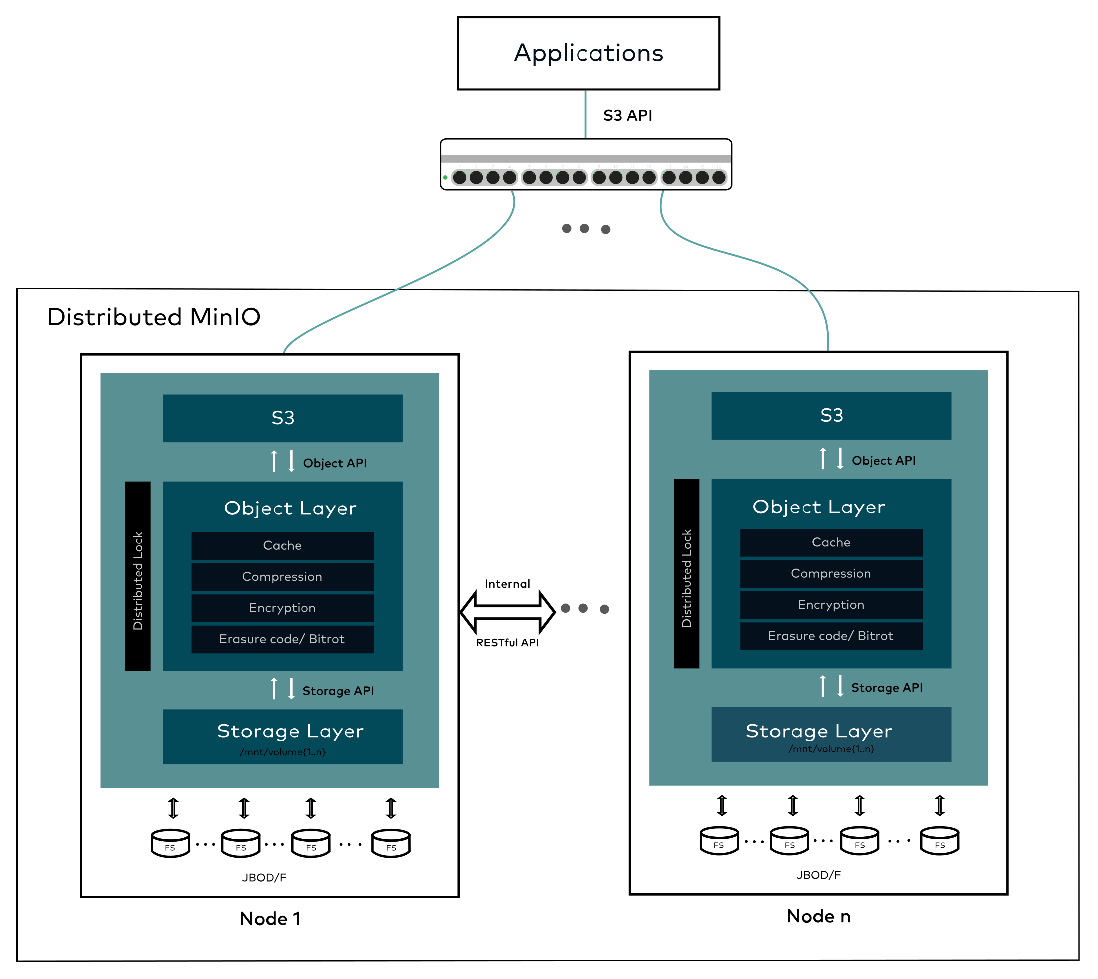
\includegraphics[angle=90, height=0.75\textheight]{obrazky-figures/minio-architecture.eps}
        \caption{Overview of MinIO cluster architecture (source: \cite{minioObjectStorage}, modified).}
        \label{fig:minio-architecture}
    \end{figure}
    \newpage


    \subsection{Event notifications}
    MinIO supports event notification for an event occurring to objects. MinIO provides Amazon S3 like events structure and API for defining which events will be published. Administrators can define bucket-level notification rules using MinIO client or provided MinIO SDK API, around which S3 events and objects will MinIO publish event notifications. MinIO Lambda Notifications are built into the MinIO object storage service and only require access to the remote notification target \cite{minioMonitoring}.

    Supported event notification targets are AMQP, Redis, MySQL, LMQTT, NATS, Apache Kafka, Elasticsearch, PostgreSQL, Webhooks, and NSQ. Figure \ref{fig:minio-monitoring} provides an overview of events triggering and event publishing in MinIO.

    Beside events occred on objects such as \texttt{s3:ObjectCreated:*} and \texttt{s3:ObjectRemoved:*}, MinIO offers event notification for access to storage \texttt{s3:ObjectAccessed:*} and event notification when bucket is created \texttt{s3:BucketCreated} and deleted \texttt{s3:BucketRemoved}.

    \begin{figure}[H]
        \centering
        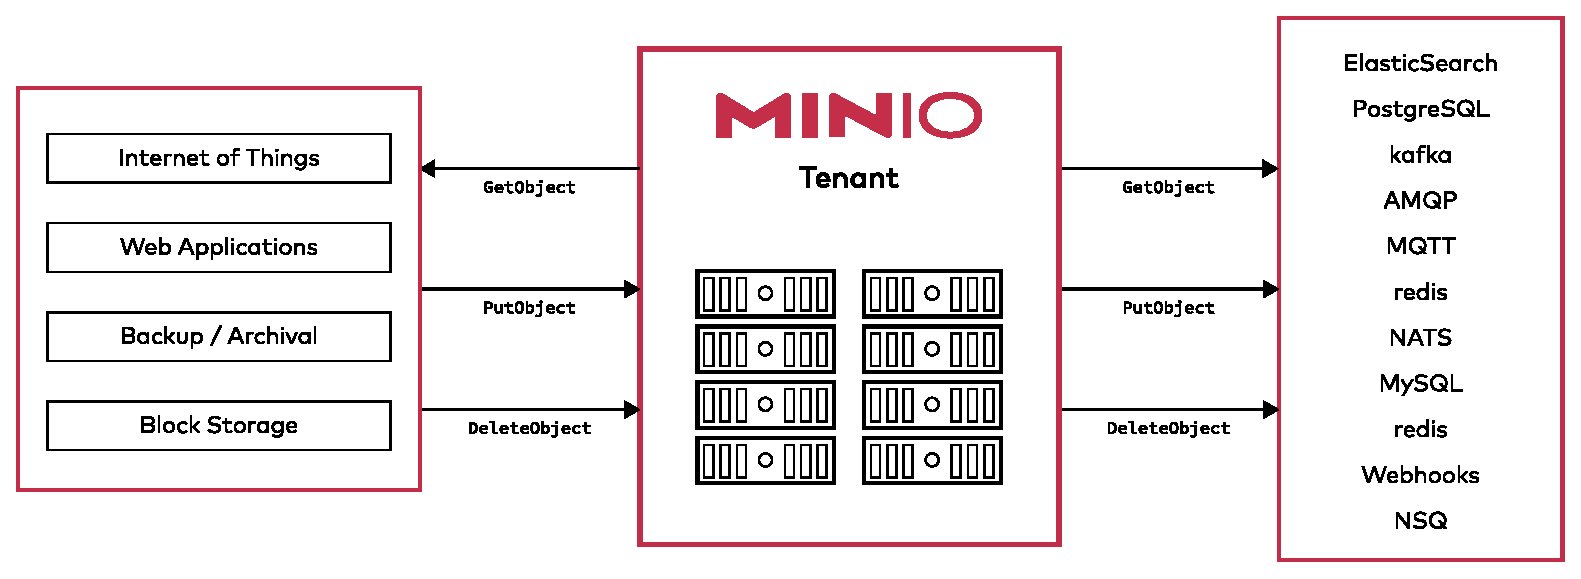
\includegraphics[width=0.96\textwidth]{obrazky-figures/minio-monitoring.eps}
        \caption{Overview of event notification in MinIO storage (source: \cite{minioMonitoring}).}
        \label{fig:minio-monitoring}
    \end{figure}


\chapter{Solution draft}\label{chap:solution}
    This chapter describes the current state of event notifications in OpenIO SDS, OpenStack Swift, and MinIO. It describes proposed solutions for OpenIO SDS and OpenStack Swift in the form of middleware and for publishing events notification from MinIO to Beanstalkd in the form of an proxy application.
\section{Current state}
    \subsection{OpenIO SDS}
    OpenIO Software-Defined storage has event-driven architecture, capable of publishing events to Beanstalkd using \textit{event-agent service} and \textit{Notify filter}.
    The main disadvantage of the current event publishing state is that configuration describing what type of events should be published is applied to the whole storage. Since OpenIO SDS is a multi-tenant space, some tenants might be interested in different events inside storage. The best use-case solution would be to let tenants decide what kind of events should be published in storage assigned to them.

    Second disadvantage is \textbf{lack of event filters}. Tenants might be interested in events involving specific objects or buckets that satisfy specific rules (e.g., object prefix, size).

    The third disadvantage is that events are published only to a beanstalkd queue. OpenIO SDS does not support any other destinations for event publishing. Since events can be used for monitoring, there should be a proper interface, allowing users to define the destination to which events will be published (e.g., Kafka, Prometheus, MySQL).

    \subsection{OpenStack Swift}
    Currently, there is support for event publishing in OpenStack Swift. For example, there is no way to detect changes in a given container except by listing its content and comparing timestamps.

    To partially solve this problem, OpenStack Swift created a specification\footnote{OpenStack Swift: Send notifications on PUT/POST/DELETE requests {\url{https://specs.openstack.org/openstack/swift-specs/specs/in_progress/notifications.html}}} of middleware that would send out notifications to users if a new object was created, metadata updated, or data has been deleted.
    Two proposed solutions\cite{swiftPatch1}\cite{swiftPatch2} lacked a standard interface for event publishing (no support for either Amazon S3 or CloudEvents), which were not accepted and are outdated.

    \subsection{MinIO}
    MinIO supports event publishing in the form of \textit{Bucket notifications}. It can inform a user when an object is created, updated, or deleted. Besides events regarding objects, MinIO provides events notifications for replication events and evens regarding creating and deleting buckets. Furthermore, MinIO allows users to configure which events will be published using the Amazon S3 event notification structure.

    MinIO offers various notification targets (e.g., MySql, Redis, Elasticsearch) but does not offer Beanstalkd as a notification target.

    Minio is open-source object storage but \textbf{does not provide custom middlewares}. However, since MinIO is implemented in the Go programming language, any custom changes (tweaks) in MinIO source code means that the whole project needs to be compiled, which can result in incompatibility in future versions of MinIO.

\section{Middleware for OpenStack Swift and OpenIO SDS}
    The goal is to create common application/middleware capable of running within OpenStack Swift and OpenIO SDS. The middleware will allow users to configure: which types of events will be published and a destination where given events will be published. Proposed middleware will be called \textbf{\texttt{ENOSS - Event Notifications in OpenStack Swift}}.

    \subsection{Location}
    For OpenIO SDS ideal place to run new middleware is inside the pipeline of event-agent. The main reason is that the event-agent has access to every event that occurs in OpenIO SDS and processes jobs in asynchronous mode, which means it will not impact the latency of client requests.

    Most of the middlewares within OpenStack Swift are placed in the Proxy server since they can react to every client request. Therefore, the new proposed middleware will also be placed inside the Proxy server pipeline.

    \subsection{Design}
    The proposed middleware heavily utilizes containers/buckets and accounts metadata. Information about which event should be published and where will be stored in metadata of upper level. For publishing events regarding objects, the configuration will be stored in a container/bucket metadata (for container/bucket events, the configuration will be stored in the account level).

    Compared to Amazon S3 Notifications, ENOSS middleware will publish events regarding containers/buckets. Furthermore, ENOSS middleware will publish events regarding access to object storage (HTTP GET/HEAD), where Amazon S3 only offers notifications about changes (PUST/POST) in a bucket.

    ENOSS middleware can be configured so that specific even types will be forbidden for publishing in whole object storage. This option could be beneficial when there are many reads from object storage, and publishing those events could significantly impact object storage performance. Therefore such event types can be disabled for whole object storage.

    Activity diagram of ENOSS middleware in container level is shown in figure \ref{fig:middlewareActivity}. Container metadata contains event notification configuration for publishing objects in a given container. Therefore the first step is to parse and validate such metadata. If the event notification configuration is not valid, then such configuration will be removed from metadata.

    The next step is deciding if the event should be published. Since metadata about event publishing is stored in the upper level, ENOSS needs to read account metadata from storage. After reading and parsing account metadata, \texttt{ENOSS} middleware checks if the event satisfies a rule in configuration retrieved from account metadata. If yes, the event will be published to a specified destination in account metadata. A similar process is done for events involving objects, except objects do not carry information about event publishing, and configuration is stored in a proper container's metadata.

    The figure \ref{fig:middlewareClassDiagram} shows simplified class diagram of ENOSS middleware. ENOSS defines \texttt{EventDestination} inteface , which simply sends created event notification to specified destination. This allow new types of event destination to be added easily in future. Class \texttt{ENOSSMiddleware} is the core of middleware. Since OpenIO Proxy is compatible with OpenStack Proxy server, there is no need to divide ENOSS middleware into subclasses.

    \begin{figure}[H]
        \centering
        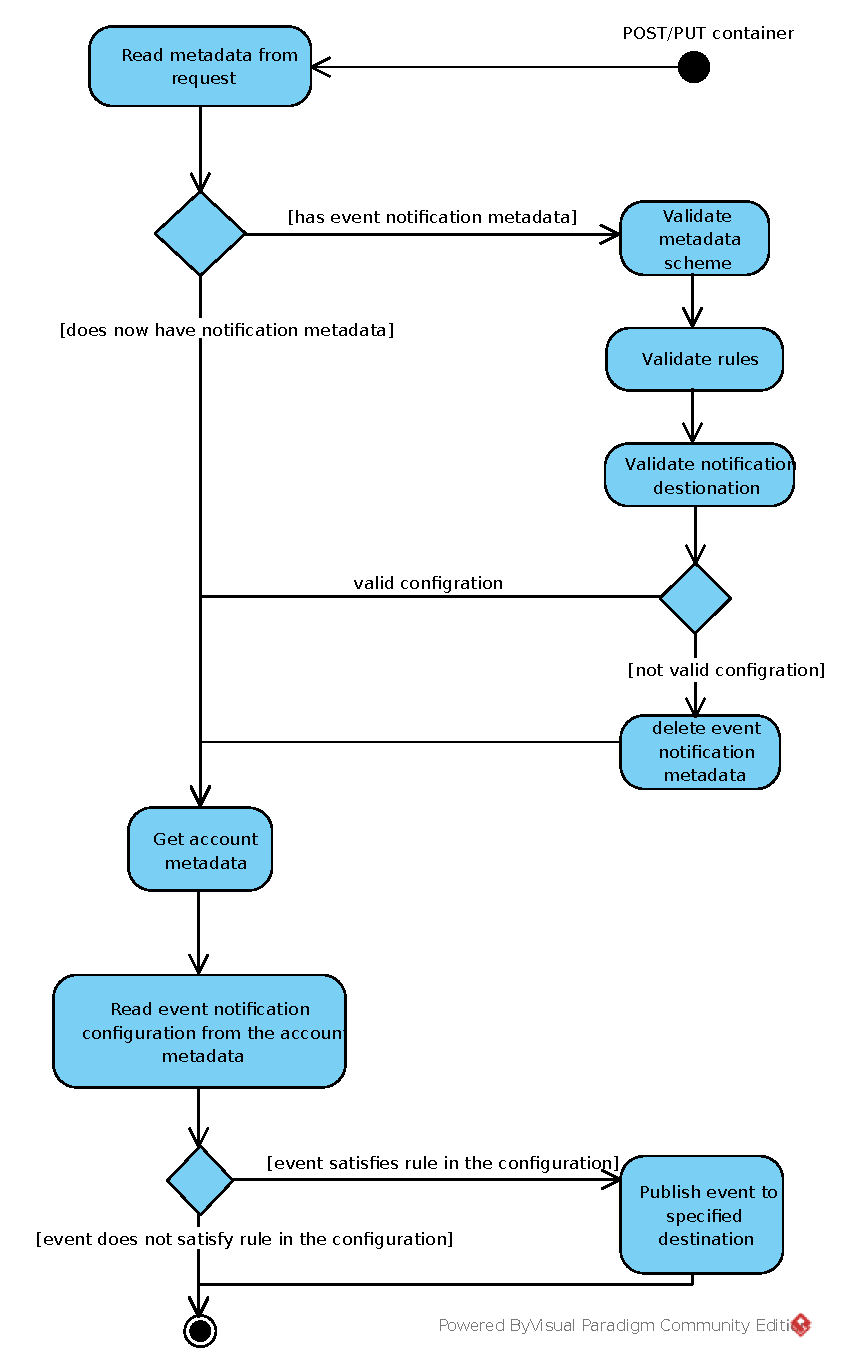
\includegraphics[width=0.9\textwidth]{obrazky-figures/middleware-activity-diagram.eps}
        \caption{Activity diagram of ENOSS middleware.}
        \label{fig:middlewareActivity}
    \end{figure}

    \begin{figure}[H]
        \centering
        %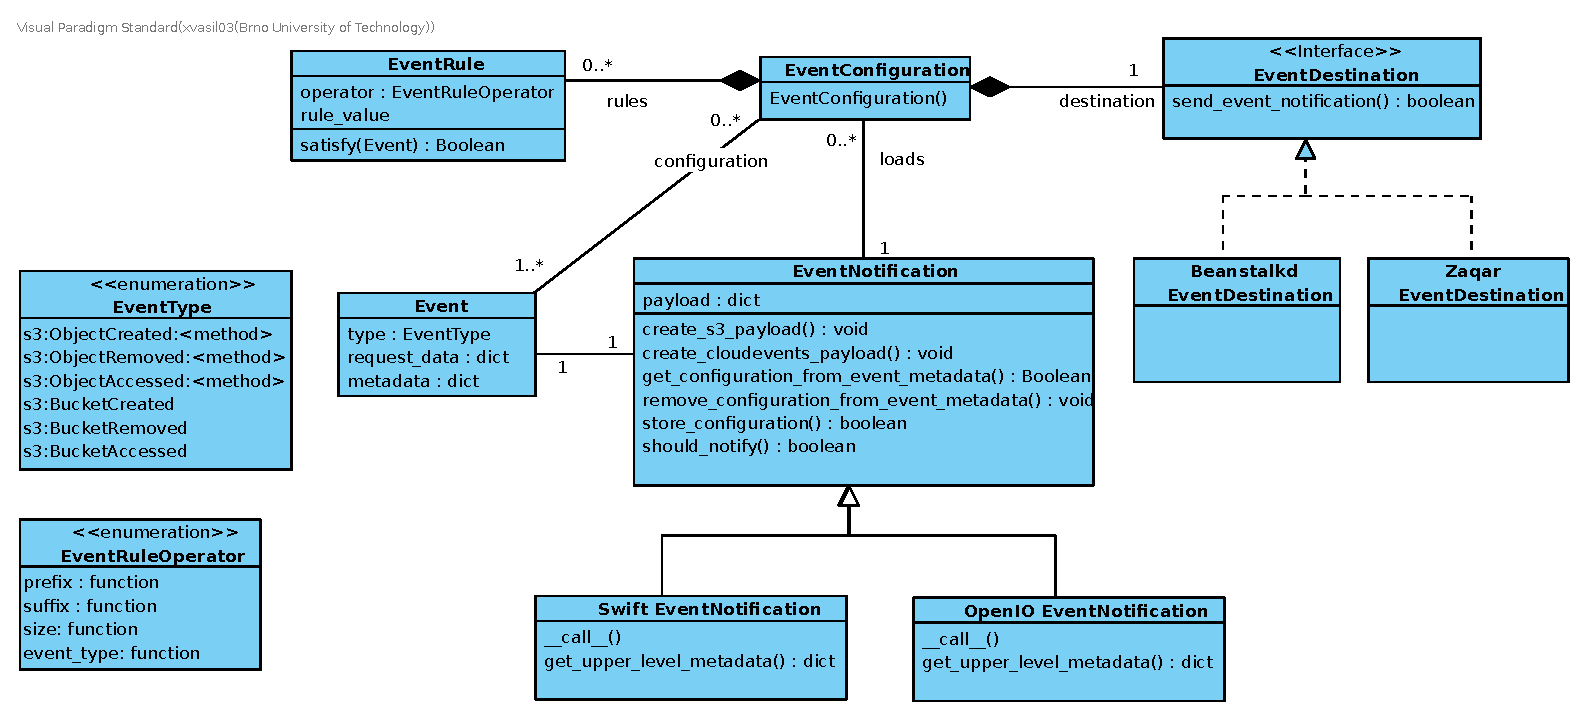
\includegraphics[angle=90,height=0.96\textheight]{obrazky-figures/eventnotifications_class_diagram.eps}
        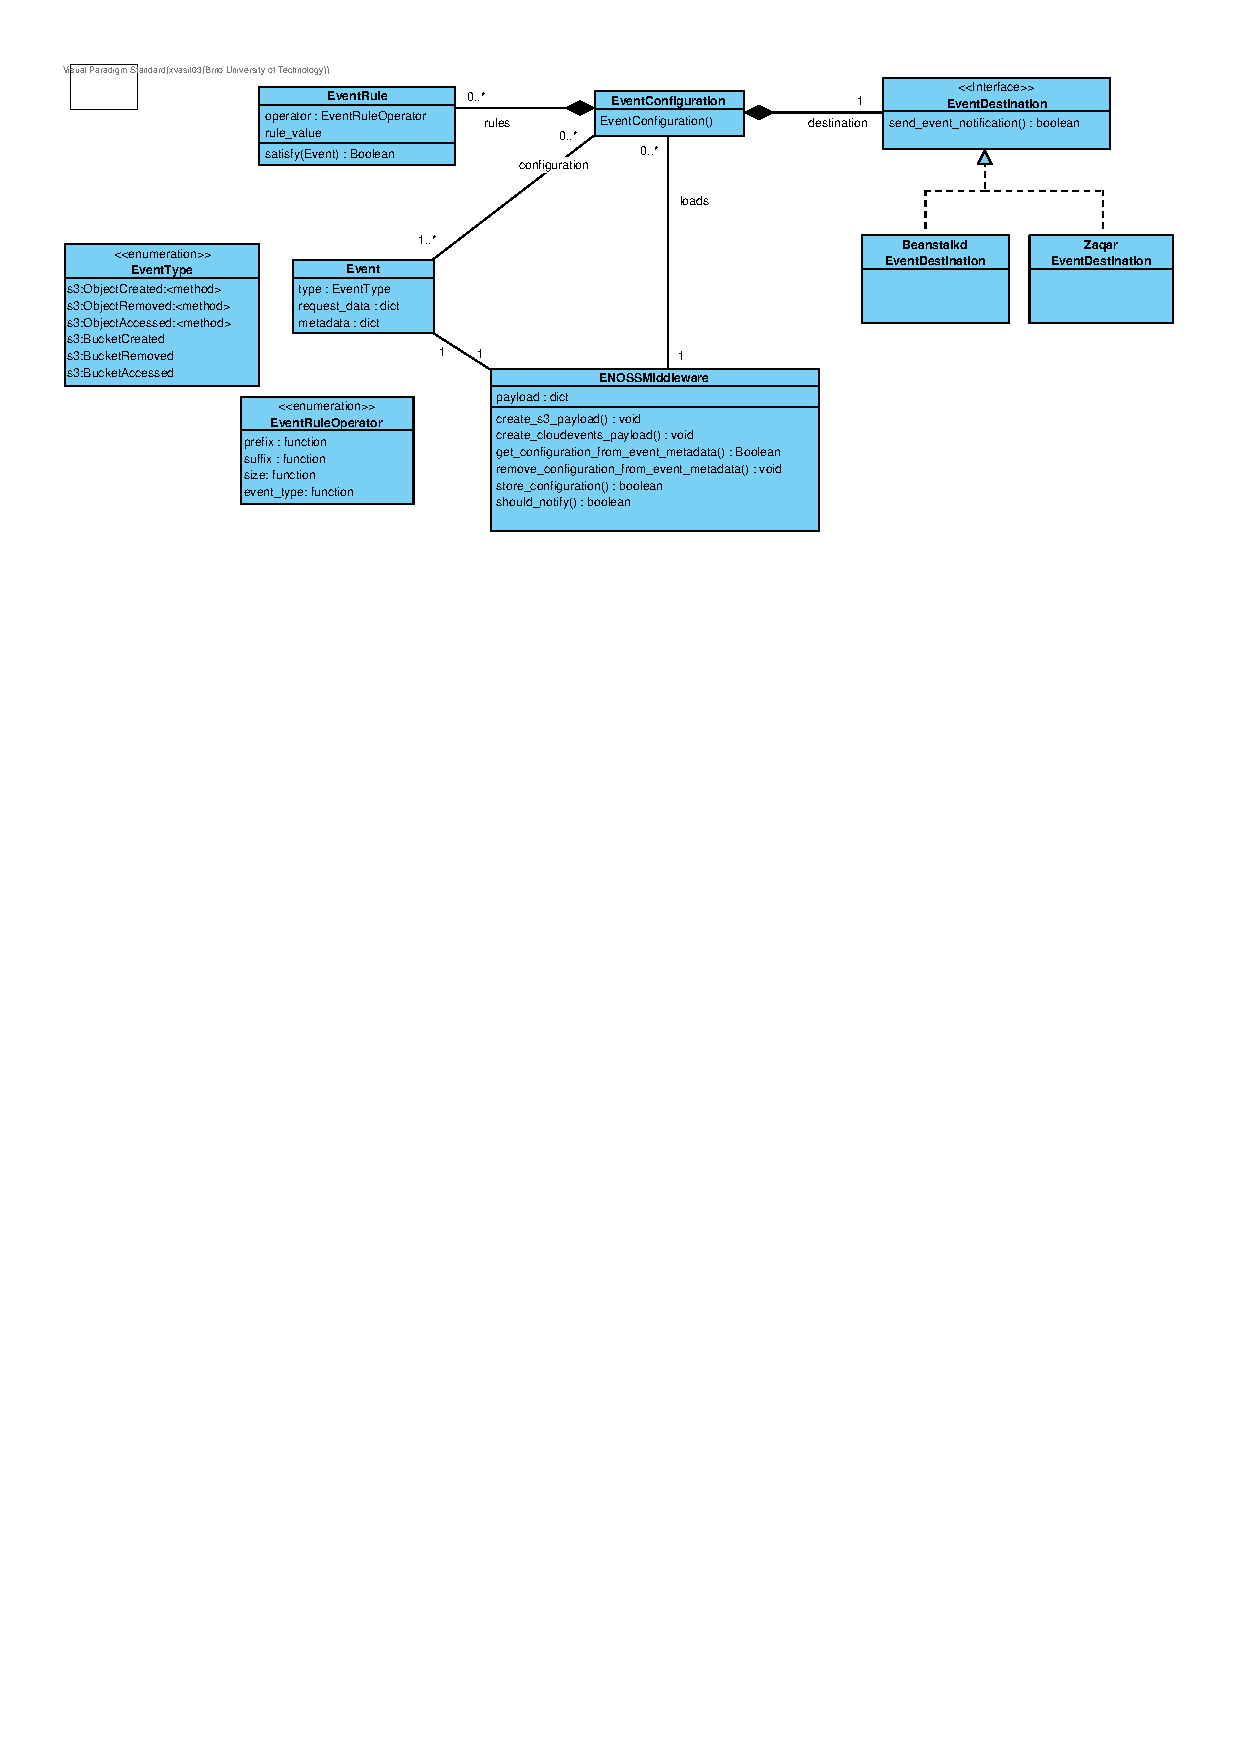
\includegraphics[angle=90,height=1\textheight]{obrazky-figures/enoss_class_diagram.pdf}
        \caption{Class diagram of ENOSS middleware.}
        \label{fig:middlewareClassDiagram}
    \end{figure}


    \subsection{Structure of published event}
    ENOSS can publish event notification in Amazon S3 like structure and in structure following CloudEvents standard. Listing \ref{lst:eventStructureCE} and \ref{lst:eventStructureS3} describes event notification structure in JSON format.

    \begin{lstlisting}[style=jsonStyle, caption=CloudEvents structure of event notification published by ENOSS middleware., label=lst:eventStructureCE]
    {
        "specversion" : "1.0",
        "type" : "event type",
        "objectstorage" : "name of object storage (swift, openiosds)",
        "source" : "URI-reference where an event occured",
        "id" : "request id",
        "time" : "the time, in ISO-8601 format when event occured",
        "datacontenttype" : "application/json",
        "data": {
            "userid": "id of user that created event",
            "useripaddress": "ip addres of user that created event",
            "requestid": "request id",
            "transactionid": "transaction id",
            "configurationid": "id configuration that trigged notification",
            "resource": {
                "name": "name of the resource that triggered event (name of an object, container or account)",
                "hash": "hash value / internal id of resource",
                "metadata": "user metadata"
            }
        }
    }
    \end{lstlisting}

    \begin{minipage}{\linewidth}
    \begin{lstlisting}[style=jsonStyle, caption=Amazon S3 structure of event notification published by ENOSS middleware., label=lst:eventStructureS3]
    {
       "Records":[
          {
             "eventVersion":"2.2",
             "eventSource":"aws:s3",
             "eventTime":"The time, in ISO-8601 format, for example, 1970-01-01T00:00:00.000Z, when an object storage finished processing the request",
             "eventName":"event-type",
             "userIdentity":{
                "principalId":"id of user who caused the event"
             },
             "requestParameters":{
                "sourceIPAddress":"ip address where request came from"
             },
             "responseElements":{
                "x-amz-request-id":"request ID"
             },
             "s3":{
                "s3SchemaVersion":"1.0",
                "configurationId":"ID found in the bucket notification configuration",
                "bucket":{
                   "name":"bucket-name",
                   "ownerIdentity":{
                      "principalId":"if od bucket owner"
                   },
                   "arn":"bucket-ARN in format arn:aws:s3:::<bucket-name>"
                },
                "object":{
                   "key":"object key/name",
                   "size":"object-size in bytes",
                   "eTag":"object eTag/hash",
                   "versionId":"object version if bucket is versioning-enabled, otherwise null",
                   "sequencer": "a string representation of a hexadecimal value used to determine event sequence, only used with PUTs and DELETEs"
                }
             }
          }
       ]
    }
    \end{lstlisting}
    \end{minipage}

    \subsection{Event Notification configuration}
    User can store event notification configuration using metadata with key \textbf{\texttt{\newline EventNotificationConfiguration}} where value is configuration.
    EvenNotifcation middleware offers Amazon S3 like structure for configuring event notifications.

    Listing \ref{lst:eventConfiguration} describes event notification configuration. \texttt{<Target>} represent targeted destination where event notifications will be sent (e.g., Beanstalkd, Elasticsearch). \texttt{<FilterKey>} is a unique name of a filter containing rules that must be satisfied in order to publish events.

    Event type takes form \texttt{s3:<Type><Action>:<Method>} and are compatible with Amazon S3 event types. Type represents resource type (object, bucket), action represent action preformed by user and can have values: \texttt{Created, Removed, Accessed}. The method represents the REST API method performed by a user: \texttt{Get, Put, Post, Delete, Copy, Head}. For example, if a new object was created, even type would be described as \texttt{\newline s3:ObjectCreated:Put}. To match event type regardless of API method assign value \texttt{*} to \texttt{<Method>}.

    \begin{minipage}{\linewidth}
    \begin{lstlisting}[style=jsonStyle, caption=Strucute of event notification configuration,    label=lst:eventConfiguration]
    {
      "<Target>Configrations": [
        {
          "Id": "configration id",
          "TargetParams": "set of key-value pairs, used specify dynamic parameters of targeted destination (e.g., name of beanstalkd tube or name of the index in Elasticsearch)",
          "Events": "array of event types that will be published",
          "PayloadStructure": "type of event notification structure: S3 or CloudEvents (default value S3)",
          "Filter": {
            "<FilterKey>": {
              "FilterRules": [
                {
                  "Name": "filter operations (i.e. prefix, sufix, size)",
                  "Value": "filter value"
                }
                ...
              ]
            }
          }
        }
        ...
      ]
    }
    \end{lstlisting}
    \end{minipage}


\section{Proxy for MinIO}
    MinIO has support for event notifications. The main problem is that it does not support Beanstalkd as an event notification destination. Since any change in MinIO source code could lead to incompatibility with future versions and with no support for custom applications/middlewares inside MinIO, the safest solution to publish event notifications from MinIO to Beanstalkd would be a proper proxy application.

    The proposing proxy application would connect to some of the supported event notifications destinations (e.g., MQTT\footnote{MQTT - extremely lightweight publish/subscribe messaging protocol {\url{https://mqtt.org/}}}), subscribe to events coming from MinIO, and forward them to Beanstalkd.

    \begin{figure}[H]
        \centering
        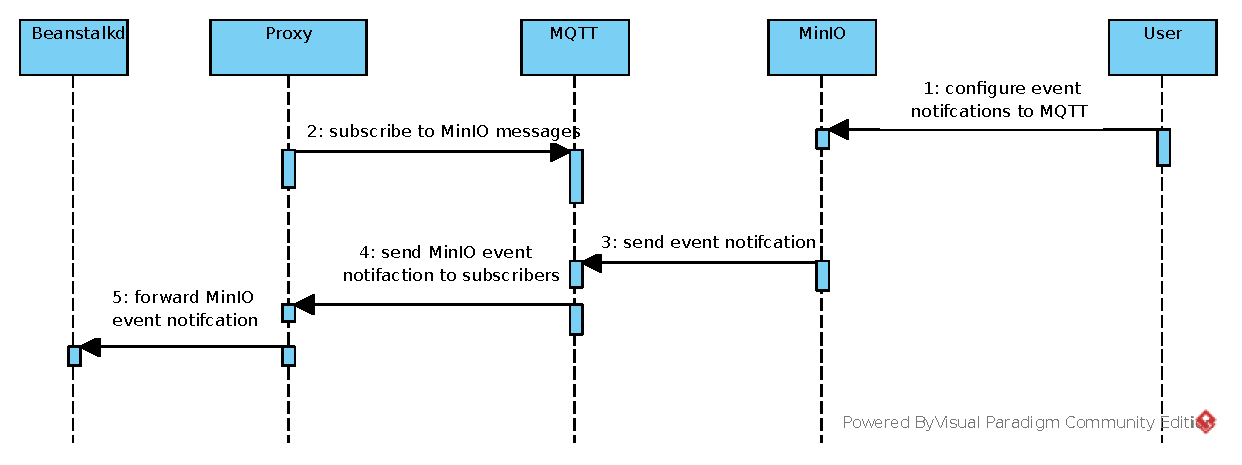
\includegraphics[angle=90,height=0.78\textheight]{obrazky-figures/minio-proxy.eps}
        %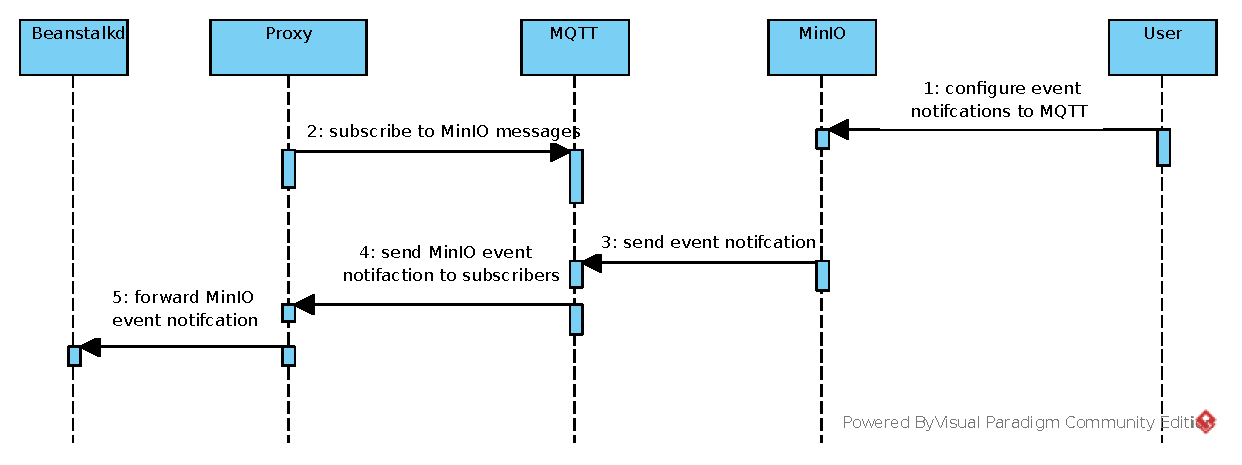
\includegraphics[width=1\textwidth]{obrazky-figures/minio-proxy.eps}
        \caption{Sequence diagram of proxy application allowing publishing events from MinIO to Beanstalkd.}
        \label{fig:minioProxy}
    \end{figure}

    Figure \ref{fig:minioProxy} shows a sequence diagram of the proposed proxy application for MQTT. The user configures MinIO event notifications using \textit{MinIO client} or \textit{MinIO SDKs}. Proxy application subscribes for MinIO messages in MQTT. Once event notification is sent from MinIO to MQTT, MQTT will send the event notification to subscribers, in this case Proxy application. Proxy application will receive a message containing an event notification from MinIO and forward it to Beanstalkd.


\chapter{Implementation}\label{chap:implementation}
    This chapter discusses the implementation of a new OpenStack middleware - ENOSS. Frist, it summarises the implementation of the central middleware and describes the new API for user communication. The chapter then describes notification configuration processing and it's validation process in ENOSS. Furthermore, this chapter covers the implementation of handlers for different types of payloads, filters, and destinations with a big emphasis on ENOSS "openness" to new custom handlers. The last part of this chapter discusses the possibility of running ENOSS inside OpenIO SDS.

    The implementation of OpenStack middleware \textbf{ENOSS} is publicly avaliable at Github\footnote{ENOSS Github repo \url{https://github.com/xvasil03/enoss}} and at official software repository for Python - Pypi\footnote{ENOSS package published on Pypi \url{https://pypi.org/project/enoss}}.


\section{ENOSS}
    ENOSS (Event notifications in OpenStack Swift) is implemented in the form of Python WSGI middleware and is located in the Proxy server pipeline. ENOSS is implemented using the flake8 coding style with the OpenStack hacking module.

    \subsection{Middleware}\label{sec:enoss-swift-section}
    Central ENOSS component is middleware located in in source file \texttt{enoss/enoss.py}. Since WSGI middleware "wraps" incoming user request and OpenStack Swift response, all informations about user request (user ip address, headers, request body, etc) and Swift response (headers, body, HTTP code, etc) are avaliable to ENOSS.

    ENOSS workflow can be divided into 6 logical stages:
    \begin{enumerate}
        \item \textbf{Storing new notification configuration} (fig. \ref{fig:enoss-stage1}) - Before incoming user request is passed on to the Proxy server pipeline, ENOSS needs to determine if user is trying to store notification configuration to OpenStack Swift. In order to allow users to store new notification configuration ENOSS offers API \texttt{POST /<account>?notification} for enabling notifications on accounts level and \texttt{POST /<account>/<container>?notification} for enabling notifications on containers level, where body of such requests contains notification configuration. Storing notification configuration to object level is forbidden and on such user request ENOSS will return HTTP Forbidden (401).

        If the incoming user request fits the specified API, ENOSS will read the request body and check if it contains a valid notification configuration. If body contains invalid configuration, ENOSS will return HTTP Bad Request (400), otherwise ENOSS will modify user request by storing notification configuration appropriate system metadata header - \texttt{"X-<type>-Sysmeta-notifications"} where \texttt{<type>} is either Account or Container. After this, the user's request will be passed down to the pipeline, and ENOSS will receive Swift's response to the user's request.

        Since system metadata can be accessed only by applications running within Swift, users cannot change notification configuration on their own (by updating metadata using POST request) and must use ENOSS API.

        ENOSS API uses the HTTP POST method; Swift will store notification configuration only if a user has write rights. This approach allows ENOSS to avoid ACL user checking and enforces that only users with write rights will be able to configure event notifications.

        \begin{figure}[H]
            \centering
            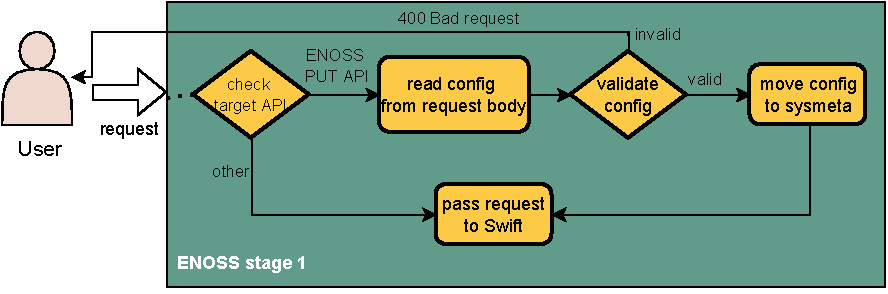
\includegraphics[width=1\textwidth]{obrazky-figures/enoss-stage1.pdf}
            \caption{ENOSS middleware stage 1 - Storing new notification configuration.}
            \label{fig:enoss-stage1}
        \end{figure}

        \item \textbf{Reading notification configurations of upper levels} (fig. \ref{fig:enoss-stage2}) - Swift processed a user's request, and ENOSS received Swift's response to the user request, which means that event occurred in Swift. The main task of this stage is to collect all notification configurations stored in the upper levels of the hierarchy. Admin notification configuration is already available (read during initialization of middleware) and remains to read configuration stored in accounts and containers level.

        Proxy server uses per request cache - internally called \textbf{infocache}, to which stores all metadata read from object storage during the processing of user's request. For reading informations(metadata) about containers and accounts Swift internally offers functions \texttt{get\_account\_info()} and \texttt{get\_container\_info()}. Those functions first check if wanted information is available in infocache, then check Memcache(if it is available), and only then do functions create another request to Swift for wanted information.

        In this specific case, metadata of upper levels are available in infocache. In addition, Admin's configuration is also available. Therefore, ENOSS does not need to create an additional request to the object storage and reads configurations from fully cached data.

        \begin{figure}[H]
            \centering
            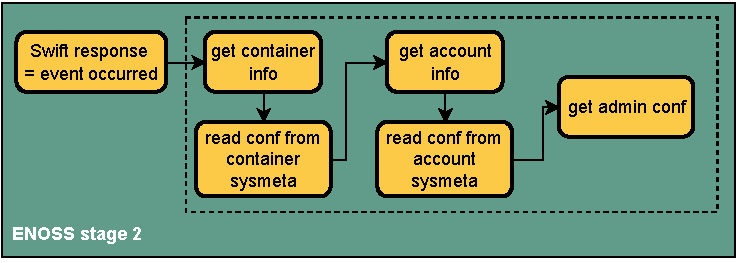
\includegraphics[width=1\textwidth]{obrazky-figures/enoss-stage2.pdf}
            \caption{ENOSS middleware stage 2 - Reading notification configurations of upper levels.}
            \label{fig:enoss-stage2}
        \end{figure}

        \item \textbf{Evaluate satisfied configurations} (fig. \ref{fig:enoss-stage3}) - Each notification configuration of the upper-level ENOSS needs to evaluate if the event should be published. In this stage, ENOSS checks if even type and filter rules are satisfied. In addition, ENOSS checks if a notification configuration allows publishing unsuccessful events (ENOSS by default publishes only successful events). It is important to note that some of the filters might need information that is not currently available(cached), resulting in an additional request to object storage.

        The results of this stage are configurations for whom an occurred event satisfies all rules and filters.

        \begin{figure}[H]
            \centering
            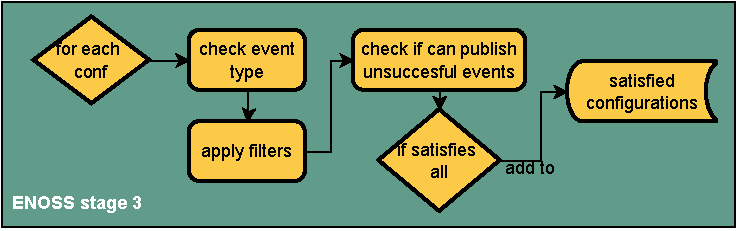
\includegraphics[width=1\textwidth]{obrazky-figures/enoss-stage3.pdf}
            \caption{ENOSS middleware stage 3 - Evaluation of satisfied configurations.}
            \label{fig:enoss-stage3}
        \end{figure}

        \item \textbf{Creating notification payload} (fig. \ref{fig:enoss-stage4-5}) - In this stage, ENOSS creates a payload of notification for the occurred event based on a specified type of payload in the notification configuration. By default payload type is AWS S3, but a user can specify other types. Like the previous stage, some information might not be available in the cache, and an additional object storage request might occur.
        \item \textbf{Sending notification} (fig. \ref{fig:enoss-stage4-5}) - Notification payload was created, and ENOSS will select a proper destination to where a notification will be sent. The target destination is specified in the notification configuration, which triggers a notification.

        \begin{figure}[H]
            \centering
            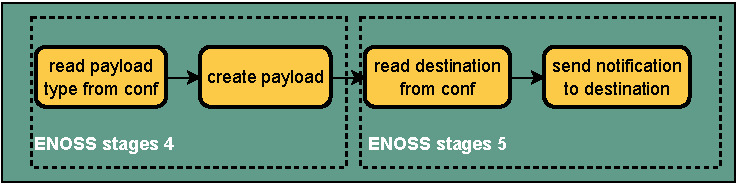
\includegraphics[width=1\textwidth]{obrazky-figures/enoss-stage4-5.pdf}
            \caption{ENOSS middleware stages 4 and 5 - Creating notification payload and sending notification to destination.}
            \label{fig:enoss-stage4-5}
        \end{figure}

        \item \textbf{Reading stored configuration} (fig. \ref{fig:enoss-stage6}) - In the last stage, ENOSS checks if a user's request was targeted towards ENOSS, i.e., if a user wanted to read stored notification configuration. For this purpose, ENOSS offers API: \texttt{POST /<account>?notification} and \texttt{POST /<account>/<container>?notification}. Suppose Swift responded successfully (HTTP 200). In that case, a user was successfully authorized to perform a read operation. Therefore ENOSS is "allowed" to send user asked information without worrying about a security breach. ENOSS will read account/container metadata using swift functions \texttt{get\_account\_info()} or \texttt{get\_container\_info()} (similarly to stage 1), and extract notification configuration from system metadata. Extracted notification configuration will be stored in a response's body of user request.

        \begin{figure}[H]
            \centering
            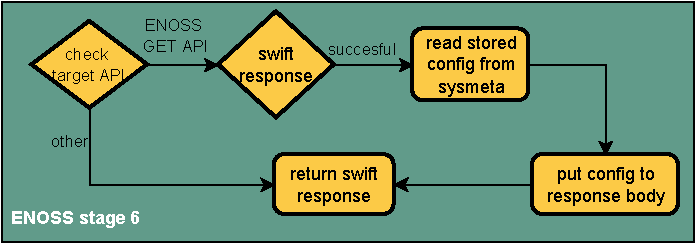
\includegraphics[width=1\textwidth]{obrazky-figures/enoss-stage6.pdf}
            \caption{ENOSS middleware stages 6 - Reading stored configration.}
            \label{fig:enoss-stage6}
        \end{figure}
    \end{enumerate}

    \textbf{Configuration} - during the runtime process, the middleware needs to validate new notification configurations, create different types of notification payloads, and send notifications to various destinations. In order to do so, the middleware needs information about available destinations and destination connection configurations. Furthermore, the middleware needs information about available payload types and the validation process of a new notification configuration. Lastly, since ENOSS allows Swift admins to publish notifications, the middleware also needs access to the admin's notification configuration.

    Part of the needed information is stored in the Proxy server's configuration. Listing \ref{lst:middlewareConfig1} shows an example of middleware configuration, where:

    \begin{itemize}
        \item \textbf{\texttt{destinations\_conf\_path}} - is a path to a configuration file containing all information needed for ENOSS to connect to various destinations (mandatory).
        \item \textbf{\texttt{use\_destinations}} - is a list of destinations (separated by a comma) that can be used during ENOSS runtime. Since ENOSS supports multiple destinations, not all of them must be used during run time. Therefore, ENOSS will create connections only to destinations specified in this list (mandatory).
        \item \textbf{\texttt{s3\_schema}} - path to file containing JSON schema used during the validation process of new notification configurations (mandatory).
        \item \textbf{\texttt{admin\_s3\_conf\_path}} - path to file containing admins notification configuration for publishing notifications (optional).
    \end{itemize}

    \lstset{
        caption=Example ENOSS middleware configuration stored in the Proxy server configuration (proxy-server.conf).,
        label=lst:middlewareConfig1
    }
    \begin{lstlisting}
    [filter:enoss]
    destinations_conf_path = /etc/swift/enoss/destinations.conf
    use_destinations=beanstalkd,elasticsearch
    s3_schema = /etc/swift/enoss/configuration-schema.json
    admin_s3_conf_path = /etc/swift/enoss/admin_s3_conf.json
    paste.filter_factory = enoss.enoss:enoss_factory
    \end{lstlisting}

    During the \textbf{initialization process}, the middleware loads destinations configuration (\texttt{destinations\_conf\_path}), uses loaded configuration to initialize destinations handlers (which create connections to destinations), loads admin's notification configuration (\texttt{admin\_s3\_conf\_path}), and initialize handlers used for the creation of different types of notification payloads.

    \subsection{Notification configuration}
    Before storing a new notification configuration, ENOSS checks if the configuration is valid. For this purpose, ENOSS uses class \textbf{\texttt{S3ConfigurationValidator}} located in \texttt{enoss/configuration\.py}. Middleware provides \texttt{S3ConfigurationValidator} with information about available destinations, payload, and new notification configuration that needs to be validated. The validation process is divided into five steps:
    \begin{enumerate}
        \item \textbf{Schema validation} - new notification configuration is validated using JSON schema validator.
        \item \textbf{Event type validation} - since a user can specify for which even types notification should be published, it is needed to validate if specified event types are supported and named correctly.
        \item \textbf{Filter validation} - a user can filter events by setting various rules that must be satisfied in order to send a notification. This step checks if specified filter rule operators are supported and if their input value is valid.
        \item \textbf{Destination validation} - \texttt{S3ConfigurationValidator} checks if for specified destinations in a new configuration exists an available destination handler in ENOSS capable of publishing notifications to specified destinations.
        \item \textbf{Payload validation} - Similar to the previous step, \texttt{S3ConfigurationValidator} checks if there is an available payload handler capable of creating a notification's payload type specified in a new notification configuration.
    \end{enumerate}

    If a new notification configuration is invalid, \texttt{S3ConfigurationValidator} will raise an  exception \textbf{\texttt{ConfigurationInvalid}}, which results in ENOSS returning HTTP Bad Request.

    Once an event occurs in Swift, middleware reads notification configurations stored in system metadata of upper levels(containers or accounts). In order to easily manipulate notification configurations, middleware represents notification configuration using class  \textbf{\texttt{S3NotifiationConfiguration}}, located in \texttt{enos/configuration.py}.

    \texttt{S3NotifiationConfiguration} offers function \texttt{get\_satisfied\_destinations()}, which for an occurred event in Swift computes destination configurations where all specified criteria for publishing notification are satisfied. This function needs to:
    \begin{itemize}
        \item Checks if occurred event type matches specified event types.
        \item Performs event filtering using specified event rules.
        \item In case of unsuccessful events (Swift response HTTP code is not 2xx), check if a user allowed publishing notification for unsuccessful events.
    \end{itemize}

    \subsection{Filters}
    ENOSS allows users to filter events using filter rules. Only events satisfying specified rules are published. ENOSS defines the interface of classes that perform various types of filtering. All filter rules classes are located in \texttt{enoss/filter\_rules/}. It is essential to notice that in some cases filter rule might need information that is not available/not cached and it can result in an additional request to Swift storage.

    \textbf{\texttt{RuleI}} - is an interface specifying class representing user-specified rules that must be satisfied in order to publish event notifications. The constructor receives a value, which is read from the notification configuration. The call method has access to all information about the request, which allows implementing rules about, e.g., user IP address, return code, object prefix/suffix/length. Function \textbf{\texttt{validate()}} is used during the validation process of new notification configurations. Its task is to validate if an input value can be used to initialize a given filter rule. This function can be used for data type checking and if an input value has a correct format.

    \begin{lstlisting}[language=Python, style=pythonStyle, caption=Interface of class representing filter rule., label=lst:enoss-rulei]
    @six.add_metaclass(abc.ABCMeta)
    class IRule(object):
        def __init__(self, value):
            self.value = value

        @abc.abstractmethod
        def __call__(self, app, request):
            raise NotImplementedError('__call__ is not implemented')

        @staticmethod
        def validate(value):
            raise NotImplementedError('validate is not implemented')
    \end{lstlisting}

    Currently, ENOSS offers the following filter rules:
    \begin{itemize}
        \item \textbf{Suffix}: input value is a string. Checks if user's request target(account/container/object) has specified suffix.
        \item \textbf{Prefix}: input value is a string. Similar to \texttt{Suffix}, except it checks targets prefix.
        \item \textbf{Maxsize}: input value is int representing size in bytes. If a request's target is an object, then checks if the object's size is not bigger than the specified size. In the case of an account or container, it checks if its used space (metadata \texttt{X-<target>-Bytes-Used}) is not bigger than the specified size.
        \item \textbf{Minsize}: input value is int representing size in bytes. Similar to \texttt{Maxsize}, except target's size must not be lower then specified size.
        \item \textbf{Contenttype}: input value is a string representing content type. If a request target is an object, then checks object type. In the case of \texttt{PUT}, \texttt{GET} or \texttt{HEAD} methods, the object's content type will be read from headers. Otherwise, an object's type will be read from object storage (if it is not in the infocache, it will result in an additional request to Swift).
        \item \textbf{Httpcodes}: input value is a list of strings representing HTTP code or group of HTTP codes (e.g. ["200", "404", "4xx"]). Checks if Swift response's HTTP code matches any of the input values. Users can use the wildcard character "x" to specify a group of HTTP codes.
        \item \textbf{Usersin}: input value is a list of strings representing a list of users. If a user who created an event in Swift is in the input list, the rule is satisfied.
        \item \textbf{Usersout}: input value is a list of strings representing a list of users. Similar to \texttt{Userin}, except rule is satisfied in user that created event is not in the input list.
    \end{itemize}

    \subsection{Notification payload}
    ENOSS is flexible regarding a payload of notifications. Notification payload might differ based on ENOSS applications and destination types to which notification should be sent. ENOSS specifies the interface of classes that create notification payload, and classes realizing defined interface are located in \texttt{enoss/payload/}.

    \textbf{PayloadI} - is an interface specifying classes used for creating notification payload. When event notifications are configured on a container or account, ENOSS sends test notifications to all specified destinations in configuration. This way, it allows users to check if they successfully configured event notifications. Method \texttt{create\_test\_payload()} is used for this purpose. One of the parameters is \texttt{request},which contains all information about the incoming request(e.g., user IP address, incoming headers) and information about Swift response(e.g., headers, status code). The \texttt{invoking\_configuration} contains information about stored notifications configuration. When an event occurs on a container/account with enabled notifications, ENOSS checks if notification for such event should be published based on event notification configuration. If yes, the method \texttt{create\_payload()} will be used to create a notification payload. Similar to filter rules, if a payload needs information that is currently not available/not in the cache, an additional request to Swift storage might occur.

    \begin{lstlisting}[language=Python, style=pythonStyle, caption=Interface of class used to create notification payload, label=lst:enoss-payloadi]
    @six.add_metaclass(abc.ABCMeta)
    class IPayload(object):
        def __init__(self, conf):
            self.conf = conf

        @abc.abstractmethod
        def create_test_payload(self, app, request, invoking_configuration):
            raise NotImplementedError('create_test_payload is not implemented')

        @abc.abstractmethod
        def create_payload(self, app, request, invoking_configuration):
            raise NotImplementedError('create_payload is not implemented')
    \end{lstlisting}

    Currently ENOSS support notification payload types:
    \begin{itemize}
        \item \textbf{S3Payload} - this class creates a notification payload compatible with Amazon AWS S3 notifications described in the listing \ref{lst:eventStructureS3}. Class is optimized to read all needed information from available sources (infocache, headers, etc.). In some cases, for example, updating objects metadata using the PUT method, some information (i.e., object size) is not available in infocache or headers. Such cases will result in an additional request to Swift storage in order to retrieve needed information.
    \end{itemize}

    \subsection{Destinations}
    ENOSS supports sending notifications to various types of destinations. Similar to filter rules and payloads, ENOSS defines interface class for this purpose. During ENOSS runtime, all available destination classes are initialized at the start of ENOSS, and their life ends with middlewares lifetime. All classes implementing destinations interface are located in \texttt{enoss/destinations/}.

    \textbf{DestinationI} - is an interface specifying classes used for sending event notifications to the desired destination. The constructor receives configuration(dict), which can contain information needed for creating a connection with the desired destination(address, port, authentication,...). Configuration is loaded from ENOSS middleware configuration, which is loaded by the Proxy server. Method \\\texttt{send\_notification()} receives notification payload(dict), and its task is to send a notification to a desired destination.

    \begin{lstlisting}[language=Python, style=pythonStyle, caption=Interface of class used for sending notification message to desired destination, label=lst:enoss-destinationi]
    @six.add_metaclass(abc.ABCMeta)
    class IDestination(object):
        @abc.abstractmethod
        def __init__(self, conf):
            raise NotImplementedError('__init__ is not implemented')

        @abc.abstractmethod
        def send_notification(self, notification):
            raise NotImplementedError('send_notification is not implemented')
    \end{lstlisting}

    \textbf{Available destinations} - ENOSS currently supports the following destinations:
    \begin{itemize}
        \item \textbf{BeanstalkdDestination} - the destination is responsible for publishing notifications to Beanstalkd work queue. The destination is implemented using Python3 client library \texttt{Greenstalk}\footnote{Greenstalk - Beanstalkd Python Client \url{https://github.com/justinmayhew/greenstalk}.}. Beanstalkd server connection configuration is stored in the destination configuration file(which is specified in ENOSS section in proxy-server.conf) under section \texttt{[beanstalkd]}. From this section, information about server address, port, and beanstalkd tube are read and used to initialize the connection using the Greenstalk library. Sending notification to Beanstalkd is relatively simple, \texttt{BeanstalkdDestination} receives notification in the form of dict, transforms it to string, and sends it to a queue using Greenstalk connection.

        \item \textbf{KafkaDestination} - the destination is responsible for publishing notifications to Apache Kafka distributed event streaming platform. The destination is implemented using Kafka Python client library \footnote{Kafka Python client \url{https://github.com/dpkp/kafka-python}}. Library provides a high-level asynchronous message producer - \textbf{\texttt{KafkaProducer}}. Similar to \texttt{BeanstalkdDestination}, \texttt{KafkaDestination} reads server configuration from the destination configuration file and reads the name of Kafka topic to which notifications will be published. Before sending a notification, \texttt{KafkaDestination} transforms the notification from dict to bytes datatype and then sends it using KafkaProducer instance.

        \item \textbf{ElasticsearchDestination} - the destination is responsible for publishing notifications to Elasticsearch search engine. The destination uses official Python Client library \footnote{Elasticsearch Python Client \url{https://www.elastic.co/guide/en/elasticsearch/client/python-api/current/index.html}}. \texttt{ElasticsearchDestination} supports HTTPS connection to Elasticsearch server. During the initialization phase, \texttt{ElasticsearchDestination} reads server connection configuration from the destination configuration file and makes a connection to Elasticsearch. After making a connection, \texttt{ElasticsearchDestination} will ping the Elasticsearch server to verify that the connection was successful. If not, an exception will be raised, and Proxy server will not be initialized. Information about targeted index and index mapping is also read from configuration. After a successful ping to the Elasticsearch server, \texttt{ElasticsearchDestination} will check if the targeted index exist. If it does not exist, an index will be created with specified index mapping(optional). In order to send a notification to Elasticsearch server, \texttt{ElasticsearchDestination} transforms the notification to a string and then uses \texttt{Elasticsearch Index API} with a specified index name.
    \end{itemize}

    \subsection{Custom filters/payloads/destinations}

    Classes that implement individual rules, payloads, and destinations can be interpreted as \textbf{handlers} that handle/perform specific jobs - create notification payloads, filter events, or send notifications to desired destinations. Each handler type has its module. For example, filter rule handlers are located in module \texttt{enoss/filter\_rules}, payload handlers in \texttt{enoss/payloads}, and destination handlers in \texttt{enoss/destination}.

    ENOSS middleware imports handlers only from specified modules; therefore, all handler classes must be imported in \texttt{\_\_init\_\_.py} of specified modules. For ENOSS middleware to assign jobs to proper handlers, ENOSS defines the following rules:
    \begin{itemize}
        \item Handlers must implement/use predefined handler interfaces. For example, inn the case of filter rules, that is \texttt{RuleI}, for payload creation \texttt{PayloadI} and for sending notification to specific destination handler class must implement interface \texttt{DestinationI}.
        \item Handler's name must be in format \textbf{\texttt{<Type><Handler suffix>}}, where handler suffix represents a type of job that handler performs. In particular, for payload creation handler suffix is \texttt{Payload}, for filter rules \texttt{Rule} and for sending notification to desired destination handler suffix is \texttt{Destination}. \texttt{<Type>} must correspond with a type of individual filter rule/payload/destination that a handler performs and is used by ENOSS during the handler selection process.
        \item All handlers must be imported in \texttt{\_\_init\_\_.py} file of a specified handler module.
    \end{itemize}

    \textbf{Handler selection} - during the initialization phase, ENOSS middleware will load all available handlers and separate them based on the type of the handler. ENOSS expects that the names of handlers match values in notification configuration. Figure \ref{fig:enoss-handler-selection} illustrates the handler section process and how names in notification configuration are connected to specific handlers. For example,  if a user-specified notification payload is "s3", ENOSS will select handler \texttt{S3Payload} from module \texttt{enoss/payloads}. The same principle is applied to filter rules and destinations. It is essential to notice that loaded handlers are used during the validation process of new notification configurations. ENOSS will declare notification configuration as invalid if the handler cannot be found.

    \begin{figure}[H]
        \centering
        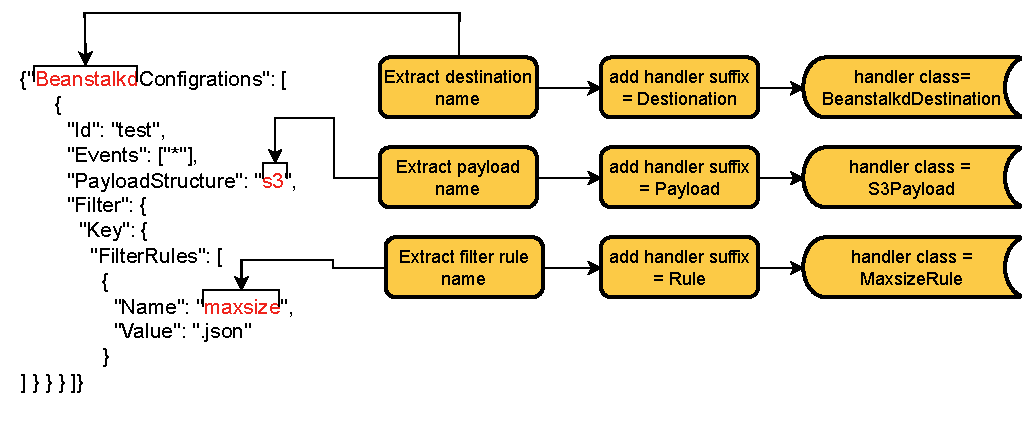
\includegraphics[width=1\textwidth]{obrazky-figures/enoss-handler-selection.pdf}
        \caption{Process of handler selection for given notification configuration.}
        \label{fig:enoss-handler-selection}
    \end{figure}

    \textbf{The creation of custom filters/payloads/destinations} can be interpreted as a creation of a new handler, and its process is simple and intuitive. A new handler must follow the specified rules(interface, name, and location). Once a new handler is implemented and imported into a proper module, a custom filter/payload/destination can be used in notification configuration using the handler selection described above.

    \subsection{OpenIO SDS compatibility}
    OpenIO SDS allows running Swift middleware using the OIO-Swift gateway. Compared to the Swift Proxy server, OpenIO SDS offers a service called \textbf{oio-proxy}. oio-proxy is, in fact, a modified Swift Proxy server that allows communication with internal object storage services needed to handle user requests. The main difference between Swift and OpenIO Proxy server is that oio-proxy is implemented using \textbf{Python 2.7} while Swift proxy runs on \textbf{Python 3}.

    ENOSS middleware, notification configuration, and validation, payload, and filter handlers implementation are compatible with Python 2 and Python 3. For this purpose, implementation was based on Python library \textbf{\texttt{six}}, which allows writing Py2/3 compatible codes.

    \textbf{The Problem} arises in the implementation of destinations handlers, which utilize third-party libraries, where compatibility with Python 2 is not guaranteed. Since support for Python 2 has officially ended, all new client libraries are mainly implemented only using Python 3.

    \textbf{Kafka} Python library is compatible with both Python 2 and Python 3. Therefore Kafka destination can be used when ENOSS is running within OpenIO SDS.

    \textbf{Beanstalkd} destination will use Python library \texttt{greenstalk} when ENOSS is running in Swift. Since \texttt{greenstalk} offers only support for Python 3, Beanstalkd needed to use another library for OpenIO SDS. For this purpose, library \texttt{pybeanstalk} was used (offers only support for Python 2). Therefore, ENOSS needs to use two different libraries in order to publish notifications to beanstalkd, from Swift and OpenIO SDS.

    \textbf{Elasticsearch} destination is compatible with Elasticsearch release version 8.2. However, this Elasticsearch release offers only Python 3 client library and is incompatible with lower versions of the Elasticsearch Python library. Therefore, when ENOSS runs in OpenIO, ENOSS cannot send notifications to Elasticsearch.

\section{MinIO proxy}
    Since publishing notifications directly from MinIO to Beanstalkd queue is not possible due to possible incompatibility in newer versions of MinIO, a proxy program is needed.

    The main idea of the proposed solution is that MinIO will publish notifications to supported destination, in this case, MQTT queue, the roxy program will read notification from MQTT and send it to Beanstalkd queue.

    Proxy program was written in Python3. For communication with MQTT, program uses Eclipse Paho library, and for communication with Beanstalkd program utilizes Greenstalk library.

    The program expects one argument - path to the configuration file in INI format. Configuration file must contain two sections:
    \begin{itemize}
        \item \textbf{beanstalkd} - information needed to connect to beanstalkd queue (address, port, and tube name).
        \item \textbf{mqtt} - information needed to connect to MQTT (broker, port, username, password, topic)
    \end{itemize}

    The program will read the configuration from the input file and then create connections to Beanstalkd and MQTT. MQTT API allows the definition of \texttt{on\_message()} callback function, which will be called whenever a new message is read from MQTT. This function is defined to read incoming message payload from MQTT and forwards it to Beanstalkd queue.

    Lastly, using function \texttt{loop\_forever()}, the program will be run in the infinite loop, while reading messages from MQTT and forwarding to the Beanstalkd queue.


\chapter{Testing, benchmark and possible applications}\label{chap:testing}
    This chapter testing ENOSS middleware to determine whether ENOSS behavior matches its specification. This process is done using two types of tests: \textbf{unit} and \textbf{functional} tests. Furthermore, this chapter explains the process of benchmarking, analyzes ENOSS latency for each stage, provides information about benchmark scenarios, and compares performance between different types of destinations.

\section{Testing}
    OpenStack Swift project provides three types of tests: unit, functional, and probe tests. The first two types(unit and functional tests) are used to verify ENOSS's correct behavior, while probe tests are not used since they are designed to test much of Swift's internal processes.
    Tests in OpenStack Swift are standardized and automated using TOX automation project\footnote{tox automation project {\url{https://tox.wiki/en/latest/}}}.

    \subsection{Unit tests}
    Swift's unit tests are designed to test small parts of the code in isolation \cite{swiftContributing123}. Unit tests check that a small selection of the code is behaving correctly. Unit tests are implemented in Python using \textbf{\texttt{unittest}} framework. ENOSS unit test is located in \texttt{test/unit/common/middleware/test\_enoss.py}.

    Since the goal of unit tests is testing in isolation, all communication with external services should be excluded. In order to achieve this, all destination handlers are replaced with mock handler \textbf{\texttt{MockDestination}}(listing \ref{lst:swift-mockdst}) using \texttt{unittest.mock.patch} decorator.

    \begin{lstlisting}[language=Python, style=pythonStyle, caption=Mock class used to replace destination handlers in unit tests., label=lst:swift-mockdst]
    class MockDestination(object):
        def __init__(self, conf):
            self.reset()

        def reset(self):
            self.state = 'notification not sent'

        def send_notification(self, notification):
            self.state = 'notification sent'
    \end{lstlisting}

    ENOSS unit test contains:
    \begin{enumerate}
        \item \textbf{Initialization test} - checks if ENOSS can be initialized.
        \item \textbf{Handlers interface test} - checks if all available handler classes implement specified interfaces.
        \item \textbf{Configuration validation tests} - checks if the validation process of notification configuration is behaving correctly. It uses various invalid configurations(unsupported event type, payload, destination, missing filter rule value, etc.) to verify the correct validation process.
        \item \textbf{New valid notification configuration} - simulates a user trying to store a new valid notification configuration to Swift using ENOSS API. Test checks if new notification configuration is stored into system metadata.
        \item \textbf{New invalid notification configuration} - simulates a user trying to store a new invalid notification configuration to Swift using ENOSS API. Test checks if return response from ENOSS is HTTP Bad request.
        \item \textbf{Reading stored notification configuration} - a user wants to read a notification configuration from object storage. Test checks if Swift response body contains notification configuration.
        \item \textbf{Invoke notification from containers level} - notification configuration is stored in the container level, and an event occurs in the object level. Test checks if notification is sent to Beanstalk queue using mocked handler \texttt{MockDestination}.
        \item \textbf{Invoke notification from account level} - notification configuration is stored in the account level, and an event occurs in the containers level. Test checks if notification is sent to Beanstalk queue using mocked \texttt{MockDestination}.
    \end{enumerate}

    \subsection{Functional tests}
    The functional Swift tests are designed to validate that the entire Swift system is working correctly from an external perspective (they are "black-box" tests). In the ENOSS testing context, functional tests are run against public Swift(and ENOSS) API endpoints. ENOSS functional test is located in \texttt{test/functional/test\_enoss.py}.

    Similar to unit tests, functional tests are implemented using \texttt{unittest} module. ENOSS functional test contains:
    \begin{enumerate}
        \item \textbf{Storing new notification configuration} - sends to Swift ENOSS API request with new valid notification configuration and checks if notification configuration is stored using additional request to Swift (using ENOSS GET API).
        \item \textbf{Deleting existing notification configuration} - deletes stored notification configuration and check if notification configuration is indeed deleted using the same principle as the previous test.
        \item \textbf{Storing invalid notification configuration} - sends to Swift ENOSS API request with invalid notification configuration, checks if Swift(ENOSS) responds with HTTP Bad request, and checks that notification configuration was not stored in Swift.
        \item \textbf{ALC test for reading stored notification configuration} - simulates an unauthorized user trying to read stored a notification configuration without read rights. Expects HTTP Unauthorized response from Swift. The exact process is repeated for an authorized user, where the test expects that the user will receive notification configuration in Swift's response body.
        \item \textbf{ALC test for storing new notification configuration} - simulates an unauthorized user trying to store a new notification configuration without write rights. Expects HTTP Unauthorized response from Swift. Then the same process does for an authorized user, where the test expects that the notification configuration will be successfully stored.
    \end{enumerate}
\section{Performance analysis}
    As described in subsection \ref{sec:enoss-swift-section}, ENOSS can be divided into 6 logical stages. In order to understand how to measure ENOSS performance, firstly, an analysis of each logical stage is needed. The analysis mainly consists of determining whether ENOSS has all needed information to perform tasks in a stage. If not, where can ENOSS obtain such information, and how long would it approximately take for ENOSS to obtain or perform the given task.

    Stages analysis:

    \begin{enumerate}
        \item \textbf{Storing new notification configuration} - information about new notification configuration is available in a user's request. ENOSS will either return HTTP Bad Request (if the configuration is invalid) or copy the configuration to the system metadata of the request. Therefore ENOSS performs this stage extremely fast, and no performance issue can occur during this stage.
        \item \textbf{Reading notification configurations of upper levels} - while Swift processes incoming request, information about account and container are read from storage and then stored in infocache. ENOSS has access to infocache and will read configurations from infocache. Therefore, no performance issues can occur in this stage as well.
        \item \textbf{Evaluate satisfied configurations} - in this stage, ENOSS performs event filtering based on stored notification configuration obtained in the previous stage. Some filter rules might need information that is not currently cached and available. For example, updating an object's metadata is done using the POST API method. The object size is not available in incoming request headers, Swift response headers, or infocache. If notification configuration contains an object size filter, ENOSS will obtain needed information using an additional request to object storage, which can cause additional latency.
        \item \textbf{Creating notification payload} - similarly to the previous stage, in order to create a notification payload, ENOSS might need information that is not cached, and to obtain such information, ENOSS will have to make an additional request to object storage.
        \item \textbf{Sending notification} - in this stage, ENOSS sends a notification to a specified destination using third-party libraries. The speed at which this task is performed depends on the type of connection with a destination (HTTP/HTTPS), the type of destination, and whether sending notifications is synchronous or asynchronous.
        \item \textbf{Reading stored configuration} - similarly to the first stage, information about stored notification configuration is available in infocache. ENOSS will copy the configuration from infocache to the response body. Therefore no performance issues can occur in this stage.
    \end{enumerate}

    Additionally, performance issues can occur during \texttt{DELETE} events. Since ENOSS creates event notifications after an event occurs, ENOSS needs to obtain information before it is deleted from object storage.

    If ENOSS obtains information from object storage, such information will be saved into infocache. This results in a \textbf{maximum of one additional request} to object storage per user's request.

    Therefore, computing ENOSS latency can be defined as:
    \texttt{\[ENOSS\_latency = time(obtaining\_needed\_information) + time(sending\_notification)\]}
    where obtaining needed information in the best scenario can be entirely from cached data, or in the worst scenario can result in \textbf{maximum one additional request} to object storage.

    \section{Experiments}
    Benchmarking was carried out on the FIT VUT university Kubernetes cluster. Each supported destination(Beanstalkd, Kafka, Elasticsearch) was created as a Kubernetes pod and service. OpenStack Swift was deployed using Nvidia Dockerfile for OpenStack Swift AIO(All in One), where Proxy, Account, Container, and Object servers are located on the same machine. OpenStack Swift pod was configured to have 16 VCPU (CPU Model: AMD EPYC 7282), 16GB RAM, and 50GB disk storage.

    Since the goal is to benchmark ENOSS middleware, which is located in the Proxy server, the Proxy server was configured to have only one worker in order to saturate the Proxy server CPU. Furthermore, in order to avoid bottlenecks on other servers, four workers were assigned(12 in total) to each of the other servers(Account, Container, and Object servers).

    The benchmarking process is done using the benchmark tool \textbf{\texttt{ssbench}}, designed by SwiftStack(Nvidia) for OpenStack Swift object storage system. \texttt{ssbench} has two main components - \textbf{ssbench-master} and \textbf{ssbench-worker}.The master component is in charge of creating and distributing benchmark jobs while workers preforms received jobs. A Benchmark test is defined using a \textbf{scenario}(sometimes called a “CRUD scenario”), which is a JSON-formatted file. The scenario contains the following information \cite{swiftSsbench123}:
    \begin{itemize}
        \item \textbf{name} - scenario's name
        \item \textbf{sizes} - list of "object size" classes. Each object size class has a name, minimum and maximum size of objects in bytes.
        \item \textbf{initia\_files} - dictionary of initial file-counts per size class. Defines probability distribution of object sizes during the benchmark run itself.
        \item \textbf{run\_seconds} - number of seconds the benchmark scenario should be run.
        \item \textbf{container\_count} - number of containers in Swift used during the benchmark run.
        \item \textbf{user\_count} - determines the maximum client concurrency during the benchmark run.
        \item \textbf{crud\_profile} - determines the distribution of each kind of CRUD operations.
    \end{itemize}

    \begin{lstlisting}[style=jsonStyle, caption=Example of ssbench scenario.]
    {
        "name": "Small test scenario",
        "sizes": [{
            "name": "tiny",
            "size_min": 4096,
            "size_max": 65536
          }, {
            "name": "small",
            "size_min": 100000,
            "size_max": 200000
        }],
        "initial_files": {
            "tiny": 100,
            "small": 10
        },
        "run_seconds": 300,
        "crud_profile": [3, 4, 2, 2],
    }
    \end{lstlisting}

    All experiments were done using one ssbench master and 5 ssbench workers. During benchmarking, information about CPU and RAM usage used by the Proxy server worker was tracked. Connections to Beanstalkd and Kafka queue are done without authorization and using an unsecured connection, while the connection with Elasticsearch is made using TLS/HTTPS connection using a CA certificate.

    \textbf{Experiment 1}: in order to fully saturate proxy CPU and avoid disk bottleneck, for this experiment ssbench scenario contains only tiny documents(size 4-6KB) and only read operations. This way, data will be serviced entirely from the buffer cache, and the disk bottleneck will be avoided. In this benchmark test, ENOSS is configured, with an admin notification configuration, to create and send notifications for all events to one destination during the benchmark test. In this scenario, ENOSS has all needed information(in infocache) and does not need to make additional requests to object storage.

    The benchmark test is repeated for each supported destination, as well as when notification configuration is not enabled, and when ENOSS is enabled in the Proxy server. Each benchmark test during this experiment was run for 60 minutes.

    Figure \ref{fig:expr1-usage} contains information about the used CPU and RAM by the Proxy server worker(where ENOSS is located). In all cases, CPU usage was saturated, and maximum output from the Proxy server was achieved. Using information about RAM usage, a conclusion can be drawn that when ENOSS is enabled, the Proxy server worker will use about 20MB more RAM for this hardware configuration.

    Table \ref{tab:expr1} contains benchmark results for this experiment. The first row(\textbf{ENOSS disabled}) in the table shows results when ENOSS is not enabled in the Proxy server pipeline. The second row(\textbf{No notifications}) contains benchmark results when ENOSS is enabled but was not configured to publish any notification. Other rows show results when ENOSS is enabled and configured to publish notifications to the specified destination.

    When ENOSS is enabled but is not configured to publish notifications, ENOSS middleware still needs to read notification configurations of upper levels(stage 2 described in subsection \ref{sec:enoss-swift-section}). Since there are no notification configurations in upper levels, ENOSS will return the received Swift response. Therefore, the latency of this example can be interpreted as the latency of the second stage. Comparing average latency when ENOSS is not enabled and when ENOSS is enabled but does not publish notifications, the statement that no performance issues can occur during reading notification configurations of upper levels is confirmed.

    Comparing the results of each supported destination, a conclusion can be drawn that the beanstalkd queue outperforms the Kafka queue. At the same time, Elasticsearch has the worst performance, partially due to the HTTPS connection. Using results when ENOSS publishes notifications and when ENOSS is not enabled, the latency of publishing notifications can be computed.

    In this experiment, when ENOSS had all needed information cached, ENOSS on average, took between 0.04(beanstalkd) and 0.16(Elasticsearch) seconds to publish a notification.

    \begin{figure}[!htb]
        \centering
        \begin{tikzpicture}[scale=0.9]
            \begin{axis}[
                xlabel=time(min),
                ylabel=CPU usage(\%),
                ymin=50,
                ymax=100,
                mark=none,
                every axis plot/.append style={thick}
            ]
            \addplot [no markers, blue] table [x=row, y=cpu] {benchmark_results/expr1/usage_beanstalkd_agg.csv};
            \addplot [no markers, red] table [x=row, y=cpu] {benchmark_results/expr1/usage_elasticsearch_agg.csv};
            \addplot [no markers, green] table [x=row, y=cpu] {benchmark_results/expr1/usage_kafka_agg.csv};
            \addplot [no markers, purple] table [x=row, y=cpu] {benchmark_results/expr1/usage_nonotif_agg.csv};
            \addplot [no markers, brown] table [x=row, y=cpu] {benchmark_results/expr1/usage_noenoss_agg.csv};
            \end{axis}
        \end{tikzpicture}
        \begin{tikzpicture}[scale=0.9]
            \begin{axis}[
                xlabel=time(min),
                ylabel=RAM(MB),
                ymin=0,
                ylabel near ticks,
                yticklabel pos=right,
                mark=none,
                every axis plot/.append style={ultra thick}
            ]
            \addplot [no markers, blue] table [x=row, y=ram] {benchmark_results/expr1/usage_beanstalkd_agg.csv};
            \addplot [no markers, red] table [x=row, y=ram] {benchmark_results/expr1/usage_elasticsearch_agg.csv};
            \addplot [no markers, green] table [x=row, y=ram] {benchmark_results/expr1/usage_kafka_agg.csv};
            \addplot [no markers, purple] table [x=row, y=ram] {benchmark_results/expr1/usage_nonotif_agg.csv};
            \addplot [no markers, brown] table [x=row, y=ram] {benchmark_results/expr1/usage_noenoss_agg.csv};
            \end{axis}
        \end{tikzpicture}
        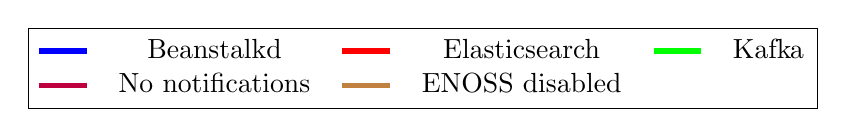
\begin{tikzpicture}
        \begin{customlegend}[legend columns=3,legend style={column sep=2ex},
                legend entries={Beanstalkd ,
                                Elasticsearch ,
                                Kafka ,
                                No notifications ,
                                ENOSS disabled,
                                }]
                \addlegendimage{no markers, line width = 2px, blue}
                \addlegendimage{no markers, line width = 2px, red}
                \addlegendimage{no markers, line width = 2px, green}
                \addlegendimage{no markers, line width = 2px, purple}
                \addlegendimage{no markers, line width = 2px, brown}
                \end{customlegend}
        \end{tikzpicture}
        \caption{Left: CPU usage by Proxy server worker during experiment 1. Right: RAM usage by Proxy server worker during experiment 1.} \label{fig:expr1-usage}
    \end{figure}

    \begin{center}
    \begin{table}[!htb]
        \begin{tabular}{|c|c|c|c|c|c|c|c|}
        \hline
        \multirow{2}{*}{Destination} & \multirow{2}{*}{\shortstack[c]{Requests\\ count}} & \multirow{2}{*}{\shortstack[c]{Requests\\ per sec}} &\multicolumn{5}{c|}{Latency(seconds)}\\
        \cline{4-8}
        & & & min & max & std dev & 95\%-idle & avg \\
        \hline
        ENOSS disabled & 1 328 729 & 369 & 0.003 & 0.926 & 0.016 & 0.026 & 0.018\\
        \hline
        No notifications & 1 159 416 & 322 & 0.003 & 1.138 & 0.018 & 0.030 & 0.021 \\
        \hline
        Beanstalkd & 1 140 780 & 316 & 0.003 & 0.861 & 0.015 & 0.031 & 0.022 \\
        \hline
        Apache Kafka & 916 787 & 254 & 0.004 & 0.953 & 0.017 & 0.039 & 0.027 \\
        \hline
        Elasticsearch(https) & 722 446 & 200 & 0.009 & 8.990 & 0.021 & 0.048 & 0.034 \\
        \hline
        \end{tabular}
        \caption{\label{tab:expr1}Benchmark results for experiment 1.}
    \end{table}
    \end{center}

    \textbf{Experiment 2}: similarly to experiment 1, the ssbench scenario contains only tiny documents, and ENOSS is configured to create notifications for all events to one destination per event. This experiment targets situations when ENOSS does not have all needed information and needs to create one additional request to Swift.

    Figure \ref{fig:expr2-usage} contains information about CPU and RAM usage by the Proxy server worker. Comparing CPU and RAM usage during this experiment with the previous experiment, a conclusion can be drawn that CPU and RAM usage remained the same. Therefore, ENOSS did not need more RAM to gather needed information from object storage.

    From table \ref{tab:expr2}, containing benchmark results for Experiment 2, a deduction can be made that making an additional request to object storage impacts latency. The worst performance occurred when ENOSS published notifications to Elasticsearch, while Beanstalkd outperformed Kafka queue, the same as the previous experiment.

    \begin{figure}[!htb]
        \centering
        \begin{tikzpicture}[scale=0.9]
            \begin{axis}[
                xlabel=time(min),
                ylabel=CPU usage(\%),
                ymin=50,
                ymax=100,
                mark=none,
                every axis plot/.append style={thick}
            ]
            \addplot [no markers, blue] table [x=row, y=cpu] {benchmark_results/expr2/usage_beanstalkd_agg.csv};
            \addplot [no markers, red] table [x=row, y=cpu] {benchmark_results/expr2/usage_elasticsearch_agg.csv};
            \addplot [no markers, green] table [x=row, y=cpu] {benchmark_results/expr2/usage_kafka_agg.csv};
            \addplot [no markers, purple] table [x=row, y=cpu] {benchmark_results/expr1/usage_nonotif_agg.csv};
            \addplot [no markers, brown] table [x=row, y=cpu] {benchmark_results/expr1/usage_noenoss_agg.csv};
            \end{axis}
        \end{tikzpicture}
        \begin{tikzpicture}[scale=0.9]
            \begin{axis}[
                xlabel=time(min),
                ylabel=RAM(MB),
                ymin=0,
                ylabel near ticks,
                yticklabel pos=right,
                mark=none,
                every axis plot/.append style={ultra thick}
            ]
            \addplot [no markers, blue] table [x=row, y=ram] {benchmark_results/expr2/usage_beanstalkd_agg.csv};
            \addplot [no markers, red] table [x=row, y=ram] {benchmark_results/expr2/usage_elasticsearch_agg.csv};
            \addplot [no markers, green] table [x=row, y=ram] {benchmark_results/expr2/usage_kafka_agg.csv};
            \addplot [no markers, purple] table [x=row, y=ram] {benchmark_results/expr1/usage_nonotif_agg.csv};
            \addplot [no markers, brown] table [x=row, y=ram] {benchmark_results/expr1/usage_noenoss_agg.csv};
            \end{axis}
        \end{tikzpicture}
        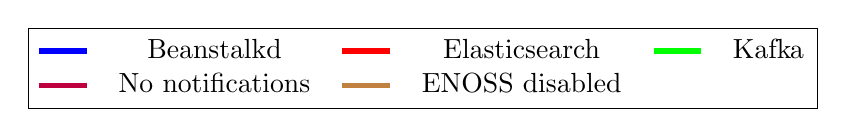
\begin{tikzpicture}
        \begin{customlegend}[legend columns=3,legend style={column sep=2ex},
                legend entries={Beanstalkd ,
                                Elasticsearch ,
                                Kafka ,
                                No notifications ,
                                ENOSS disabled,
                                }]
                \addlegendimage{no markers, line width = 2px, blue}
                \addlegendimage{no markers, line width = 2px, red}
                \addlegendimage{no markers, line width = 2px, green}
                \addlegendimage{no markers, line width = 2px, purple}
                \addlegendimage{no markers, line width = 2px, brown}
                \end{customlegend}
        \end{tikzpicture}
        \caption{Left: CPU usage by Proxy server worker during experiment 2. Right: RAM usage by Proxy server worker during experiment 3.} \label{fig:expr2-usage}
    \end{figure}

    \begin{center}
    \begin{table}[!htb]
        \begin{tabular}{|c|c|c|c|c|c|c|c|}
        \hline
        \multirow{2}{*}{Destination} & \multirow{2}{*}{\shortstack[c]{Requests\\ count}} & \multirow{2}{*}{\shortstack[c]{Requests\\ per sec}} &\multicolumn{5}{c|}{Latency(seconds)}\\
        \cline{4-8}
        & & & min & max & std dev & 95\%-idle & avg \\
        \hline
        ENOSS disabled & 1 328 729 & 369 & 0.003 & 0.926 & 0.016 & 0.026 & 0.018\\
        \hline
        No notifications & 1 159 416 & 322 & 0.003 & 1.138 & 0.018 & 0.030 & 0.021 \\
        \hline
        Beanstalkd & 732 845 & 203 & 0.006 & 0.638 & 0.016 & 0.046 & 0.034 \\
        \hline
        Apache Kafka & 570 528  & 158 & 0.007 & 0.909 & 0.018 & 0.056 & 0.043 \\
        \hline
        Elasticsearch(https) & 498 556 & 138 & 0.011 & 0.870 & 0.023 & 0.069 & 0.050 \\
        \hline
        \end{tabular}
        \caption{\label{tab:expr2}Benchmark results for experiment 2.}
    \end{table}
    \end{center}

    \textbf{Experiment 3}: this experiment aims to simulate real-life usage of OpenStack Swift object storage. Scenario contains tiny(1-10KB), small(100KB) and medium(1MB) objects, CRUD operations distribution is 36\% create, 27 \% read, 18\% update and 18\% delete, where 52\% of operations were with tiny objects, 35\% with small and 13\% with medium objects.  The duration of each benchmark test during this experiment is 30 minutes.

    In figure \ref{fig:expr3-usage} can be seen that no CPU saturation was achieved since the scenario involves larger objects and non-read operations, which led to disks(and other components) bottlenecks. Figure \ref{fig:expr3-usage} shows that during benchmark tests, when ENOSS was enabled, CPU usage increased. Computing(and then comparing) average CPU usage during different benchmark tests in this experiment was discovered that CPU usage increases from 10 to 13\% when ENOSS is enabled.

    In table \ref{tab:expr3} can be seen that the latency trend is similar to other experiments. Again, Beanstalkd shows the best performance and outperforms Kafka queue, while Elasticsearch is last.

    \begin{figure}[h]
        \centering
        \begin{tikzpicture}[scale=0.9]
            \begin{axis}[
                xlabel=time(min),
                ylabel=CPU usage(\%),
                ymin=0,
                ymax=100,
                mark=none,
                every axis plot/.append style={thick}
            ]
            \addplot [no markers, blue] table [x=row, y=cpu] {benchmark_results/expr3/usage_beanstalkd_agg.csv};
            \addplot [no markers, red] table [x=row, y=cpu] {benchmark_results/expr3/usage_elasticsearch_agg.csv};
            \addplot [no markers, green] table [x=row, y=cpu] {benchmark_results/expr3/usage_kafka_agg.csv};
            \addplot [no markers, purple] table [x=row, y=cpu] {benchmark_results/expr3/usage_nonotif_agg.csv};
            \addplot [no markers, brown] table [x=row, y=cpu] {benchmark_results/expr3/usage_noenoss_agg.csv};
            \end{axis}
        \end{tikzpicture}
        \begin{tikzpicture}[scale=0.9]
            \begin{axis}[
                xlabel=time(min),
                ylabel=RAM(MB),
                ymin=0,
                ylabel near ticks,
                yticklabel pos=right,
                mark=none,
                every axis plot/.append style={ultra thick}
            ]
            \addplot [no markers, blue] table [x=row, y=ram] {benchmark_results/expr3/usage_beanstalkd_agg.csv};
            \addplot [no markers, red] table [x=row, y=ram] {benchmark_results/expr3/usage_elasticsearch_agg.csv};
            \addplot [no markers, green] table [x=row, y=ram] {benchmark_results/expr3/usage_kafka_agg.csv};
            \addplot [no markers, purple] table [x=row, y=ram] {benchmark_results/expr3/usage_nonotif_agg.csv};
            \addplot [no markers, brown] table [x=row, y=ram] {benchmark_results/expr3/usage_noenoss_agg.csv};
            \end{axis}
        \end{tikzpicture}
        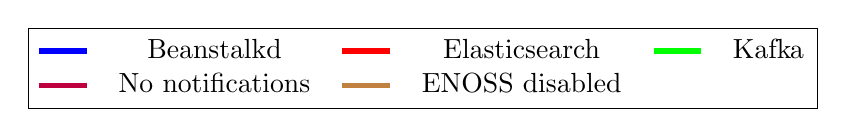
\begin{tikzpicture}
        \begin{customlegend}[legend columns=3,legend style={column sep=2ex},
                legend entries={Beanstalkd ,
                                Elasticsearch ,
                                Kafka ,
                                No notifications ,
                                ENOSS disabled,
                                }]
                \addlegendimage{no markers, line width = 2px, blue}
                \addlegendimage{no markers, line width = 2px, red}
                \addlegendimage{no markers, line width = 2px, green}
                \addlegendimage{no markers, line width = 2px, purple}
                \addlegendimage{no markers, line width = 2px, brown}
                \end{customlegend}
        \end{tikzpicture}
        \caption{Left: CPU usage by Proxy server worker during experiment 3. Right: RAM usage by Proxy server worker during experiment 3.} \label{fig:expr3-usage}
    \end{figure}

    \begin{center}
    \begin{table}[!htb]
        \begin{tabular}{|c|c|c|c|c|c|c|c|}
        \hline
        \multirow{2}{*}{Destination} & \multirow{2}{*}{\shortstack[c]{Requests\\ count}} & \multirow{2}{*}{\shortstack[c]{Requests\\ per sec}} &\multicolumn{5}{c|}{Latency(seconds)}\\
        \cline{4-8}
        & & & min & max & std dev & 95\%-idle & avg \\
        \hline
        ENOSS disabled & 223 618 & 124 & 0.004 & 6.239 & 0.044 & 0.097 & 0.039\\
        \hline
        No notifications & 204 998 & 113 & 0.004 & 3.682 & 0.042 & 0.105 & 0.043 \\
        \hline
        Beanstalkd & 204 894 & 113 & 0.004 & 3.866 & 0.046 & 0.102 & 0.042 \\
        \hline
        Apache Kafka & 193 471 & 107 & 0.004 & 5.104 & 0.047 & 0.104 & 0.045 \\
        \hline
        Elasticsearch(https) & 172 672 & 95 & 0.009 & 1.924 & 0.049 & 0.104 & 0.050 \\
        \hline
        \end{tabular}
        \caption{\label{tab:expr3}Benchmark results for experiment 3.}
    \end{table}
    \end{center}

    Experiments results tracking average request count per second, and latency are combined and displayed in figures \ref{fig:expr-combined-reqs} and \ref{fig:expr-combined-latency}. From provided results can be concluded that:
    \begin{itemize}
        \item Beanstalkd has the best performance, while Elasticsearch is the slowest.
        \item ENOSS has a relatively small impact on latency for users that do not have enabled notifications.
        \item Making an additional request to Swift, in order to retrieve needed information, increases latency (in these experiments by 12-16 ms).
        \item Creating notification for each event in Swift resulted in only a 10-15 \% performance decrease for Beanstalk and Kafka queue.
    \end{itemize}

    \begin{figure}[!htb]
        \begin{tikzpicture}
            \begin{axis}[
                    ybar,
                    bar width=.5cm,
                    width=1\textwidth,
                    height=.5\textwidth,
                    legend style={at={(0.5,1)},
                        anchor=north,legend columns=-1},
                    symbolic x coords={expr0, experiment1, experiment2, experiment3, expr4},
                    xtick=data,
                    nodes near coords,
                    nodes near coords align={vertical},
                    ymax=450,
                    ymin=0,
                    xmin=expr0,
                    xmax=expr4,
                    ylabel={Requests count},
                ]
                \addplot table[x=expr,y=beanstalkd]{benchmark_results/experiments_reqs_per_sec.txt};
                \addplot table[x=expr,y=elasticsearch]{benchmark_results/experiments_reqs_per_sec.txt};
                \addplot table[x=expr,y=kafka]{benchmark_results/experiments_reqs_per_sec.txt};
                \addplot table[x=expr,y=no_notif]{benchmark_results/experiments_reqs_per_sec.txt};
                \addplot table[x=expr,y=no_enoss]{benchmark_results/experiments_reqs_per_sec.txt};
                \legend{Beanstalkd, Elasticsearch, Kafka, No notifications, ENOSS disabled}
            \end{axis}
        \end{tikzpicture}
        \caption{Combined experiments results tracking average number of requests per second. Bigger value is better.}
        \label{fig:expr-combined-reqs}
    \end{figure}

    \begin{figure}[!htb]
        \begin{tikzpicture}
            \begin{axis}[
                    ybar,
                    bar width=.5cm,
                    width=1\textwidth,
                    height=.5\textwidth,
                    legend style={at={(0.5,1)},
                        anchor=north,legend columns=-1},
                    symbolic x coords={expr0, experiment1, experiment2, experiment3, expr4},
                    xtick=data,
                    nodes near coords,
                    nodes near coords align={vertical},
                    ymax=60,
                    xmin=expr0,
                    xmax=expr4,
                    ylabel={Latency(ms)},
                ]
                %\addplot table[x=interval,y=carT]{\mydata};
                \addplot table[x=expr,y=beanstalkd]{benchmark_results/experiments_latency.txt};
                \addplot table[x=expr,y=elasticsearch]{benchmark_results/experiments_latency.txt};
                \addplot table[x=expr,y=kafka]{benchmark_results/experiments_latency.txt};
                \addplot table[x=expr,y=no_notif]{benchmark_results/experiments_latency.txt};
                \addplot table[x=expr,y=no_enoss]{benchmark_results/experiments_latency.txt};
                \legend{Beanstalkd, Elasticsearch, Kafka, No notifications, ENOSS disabled}
            \end{axis}
        \end{tikzpicture}
        \caption{Combined experiments results tracking latency. Smaller value is better.}
        \label{fig:expr-combined-latency}
    \end{figure}
    \section{Use cases and applications}
    ENOSS has multiple use cases. Some of possible use case scenarios where ENOSS can be applied are:

    \begin{itemize}
        \item \textbf{Event monitoring and alerting} - ENOSS can be expanded to publish notifications to more sophisticated event monitoring services with alerting (like Prometheus).

        \item \textbf{Anomaly detection} - since ENOSS is capable of publishing unsuccessful events, using filter \textbf{httpcodes} admin can set ENOSS to publish notifications about events involving internal errors (HTTP code 5xx) or any other unsuccessful HTTP codes.

        \item \textbf{Data theft detection} - user has a designated container for sensitive data. The container owner can "tell" ENOSS which users should have access to the container, and if some unknown users, that are not in the list of users specified by the container's owner, somehow gain access to the container, then ENOSS will publish a notification about such event.

        \item \textbf{Data theft prevention} - user configures ENOSS to publish unauthorized events, which can result in the detection of the possible attempt of data theft.

        \item \textbf{Postprocessing} - user wants to search stored data using their metadata. The user configures ENOSS to publish events that store, modify and delete data in object storage. The destination of published events would be Elasticsearch or some other custom destination capable of full-text search.
    \end{itemize}

\chapter{Conclusion}\label{chap:conclusion}
    This thesis aimed to provide a way for users to retrieve information about events occurring in parts of object storage that they own/have access to. The primary destination for such information was the Beanstalkd queue. This goal was achieved by creating OpenStack Swift middleware called ENOSS(Event Notifications in OpenStack Swift).

    ENOSS allows users to specify which event types should be published. Furthermore, ENOSS offers users additional even filtering using filter rules such as prefix, suffix, size, returned HTTP status code, and users list. All these filters, including event type, can be combined, allowing users to specify events that need to be published more precisely.

    ENOSS offers several destinations to which notifications can be published. From popular stream-processing platform Apache Kafka to lightweight and extremely fast Beanstalkd working queue. ENOSS also supports publishing notifications to Elasticsearch, with many applications (from simple logging to more complex usage like indexing metadata).

    Another ENOSS feature is the support of different payload types. Since ENOSS supports multiple destinations and has multiple applications, notification payloads may differ based on ENOSS usage.

    One of the key advantages and ENOSS features is support for custom destinations, payloads, and filters.
    In addition, ENOSS offers effortless creation and integration of new destinations, payloads, and filters using predefined interfaces and rules.

    ENOSS configuration and notification payload are compatible with AWS S3 Event Notification. This key feature will allow future users to easily manipulate ENOSS since S3 Notifications are well documented and widely used. Additionally, OpenStack Swift and OpenIO SDS will be more competitive in the market since notifications were not supported in these object storages until now. S3 compatibility will also allow more accessible transition users from AWS S3 to OpenStack Swift or OpenIO SDS.

    Benchmarking showed that even during stress tests when all events were published, sending notifications had a pretty minor impact on object storage performance. In the worst-case scenario, ENOSS needs to make an additional request to object storage to decide if an event should be published or to create a notification payload. From the experiment results simulating everyday daily use of object storage, it was concluded that publishing notifications had a pretty minor impact on latency - between 3ms (for Beanstalkd queue) and 11ms for Elasticsearch.

    The work of the thesis was presented at the student conference of innovation, technology, and science Excel@FIT2022 under the name "ENOSS - Event Notifications in OpenStack Swift". The work received an award by the expert commission for the beneficial extension of the platform OpenStack.

    Possible future work and ENOSS improvements include creating support for new destinations(MQTT, Redis, NSQ), payloads, and filters. One of the current ENOSS limitations is that some supported destinations can publish notifications to a single server address. Support for secondary destination servers would be beneficial.


%=========================================================================
